\documentclass[12pt,a4paper,openany]{ctexbook}%%%%字体大小默认为12pt(小四)
%\documentclass[12pt,a4paper,oneside]{ctexbook}%%%%字体大小默认为12pt(小四)
% \usepackage{subfigure}
\usepackage[sort]{gbt7714}
% \citestyle{numbers}
\newtheorem{thm}{定理}
%%%%%%图片
\usepackage{graphicx}
\usepackage{subfigure}
%%%%%%%图形和表格控制宏包
\usepackage{rotating}
%%%%%%%图形和表格标题
\usepackage{caption2}
%%%%%%%图文混排
%\usepackage{floatflt}
%%%%%%%表格toprule midrule bottomrule
\usepackage{booktabs}
%%%表格斜线
\usepackage{diagbox}
%%%%\Xhline{length}\Xcline{c1-c2}{length}
\usepackage{makecell}

%%%%%%图形表格浮动防止到下一个section
%\usepackage[section]{placeins}
% 定制表格和图形的多行标题行距
\usepackage{setspace}
\usepackage{multirow}

%%%%%%超链接
\usepackage[colorlinks,linkcolor=black,anchorcolor=black,citecolor=black,CJKbookmarks=Ture]{hyperref}
%%%%%%数学
\usepackage{amsmath}
\usepackage{amssymb}
%%%%%%物理
\usepackage{physics}
%%%%%%控制目录
\usepackage{titletoc}
%%%%%%控制字体大小的宏包
\usepackage{type1cm}
%%%%%%bm 加粗
\usepackage{bm}
%%%%%%页眉页脚
\usepackage{fancyhdr}
%%%%%%%版面
\usepackage[left=2.5cm,right=2cm,top=2.5cm,bottom=2cm]{geometry}
%章节标题格式设置
\usepackage{titlesec}
%\usepackage{xeCJK}
%%%%enumerate 编号
%\usepackage{enumerate}
\usepackage{wallpaper}
% \usepackage{cite}
%%%字母上斜线
\usepackage{slashed}
%\usepackage{url}
%\usepackage[toc,page]{appendix}
\usepackage{appendix}
%%
%\usepackage{subcaption}
%\usepackage{cleveref}
\usepackage{tocvsec2}
%%%
\usepackage{siunitx}
\usepackage{enumerate}
%%%% include pdf file
\usepackage{pdfpages}
%%%toc
\usepackage{titletoc}
\usepackage{picinpar}

\usepackage{wrapfig}
% \usepackage[backend=biber,style=gb7714-2015,doi=false,url=false,eprint=false,gbnamefmt=lowercase]{biblatex}
% \addbibresource[location=local]{b.bib}
\usepackage{tikz}

%%%%%%%%%%%字体大小
\newcommand{\chuhao}{\fontsize{42pt}{\baselineskip}\selectfont}
\newcommand{\xiaochuhao}{\fontsize{36pt}{\baselineskip}\selectfont}
\newcommand{\yihao}{\fontsize{26pt}{\baselineskip}\selectfont}
\newcommand{\xiaoyihao}{\fontsize{24pt}{\baselineskip}\selectfont}
\newcommand{\erhao}{\fontsize{22pt}{\baselineskip}\selectfont}
\newcommand{\xiaoerhao}{\fontsize{18pt}{\baselineskip}\selectfont}
\newcommand{\sanhao}{\fontsize{16pt}{\baselineskip}\selectfont}
\newcommand{\xiaosanhao}{\fontsize{15pt}{\baselineskip}\selectfont}
\newcommand{\sihao}{\fontsize{14pt}{\baselineskip}\selectfont}
\newcommand{\xiaosihao}{\fontsize{12pt}{\baselineskip}\selectfont}
\newcommand{\wuhao}{\fontsize{10.5pt}{\baselineskip}\selectfont}
\newcommand{\xiaowuhao}{\fontsize{9pt}{\baselineskip}\selectfont}
\newcommand{\liuhao}{\fontsize{7.5pt}{\baselineskip}\selectfont}
\newcommand{\xiaoliuhao}{\fontsize{6.5pt}{\baselineskip}\selectfont}
\newcommand{\qihao}{\fontsize{5.5pt}{\baselineskip}\selectfont}
\newcommand{\xiaoqihao}{\fontsize{5pt}{\baselineskip}\selectfont}
%%%%%%%%%%%%目录
% 定义章节标题格式
% 带编号的章节标题
% 带编号的章节标题


% 定义目录内容格式
% \titlecontents{chapter}[0pt]
%   {\vspace{1ex}\bfseries\sffamily\sihao}
%   {\thecontentslabel\quad}
%   {}{\hfill\contentspage}
% \titleformat{\chapter}[display]
%   {\sffamily\xiaosanhao\bfseries}{\chaptertitlename\ \thechapter}{1em}{\vspace{1.5ex}}
% % 不带编号的章节标题
% \titleformat{name=\chapter,numberless}[display]
%   {\sffamily\xiaosanhao\bfseries}{\titlerule[1pt]\vspace{1ex}\filcenter}{}{}


% 定义目录内容格式
% \titlecontents{chapter}[0pt]
%   {\vspace{1ex}\bfseries\sffamily\sihao}
%   {\thecontentslabel\quad}
%   {}{\hfill\contentspage}
% \titlecontents{chapter}[0pt]{\vspace{0.5\baselineskip}\bfseries\sffamily\sihao}
% {\thecontentslabel\quad}{}{\hfill\contentspage}
%\setcounter{tocdepth}{3}
%\setcounter{secnumdepth}{3}
\dottedcontents{chapter}[1.8cm]{\fontsize{14pt}{14pt}\selectfont\heiti\vspace{0.5cm}}{4.0em}{10pt}
%\dottedcontents{section}[0.8cm]{}{1.8em}{5pt}
%\dottedcontents{subsection}[1.9cm]{}{2.7em}{5pt}
%\dottedcontents{subsubsection}[2.86cm]{}{3.4em}{5pt}
%====================== 定制图形和表格标题样式 =====================%
%---------------------- 定制图形和表格标题格式 ---------------------%
\renewcommand{\captionlabeldelim}{} %定义如  "图(表)2: 示例" 中的间隔符号,如 ":" ,这里定义为空
\renewcommand{\captionlabelsep}{\hspace{1em}} %定义图表编号与标题间的间隔距离
\renewcommand{\captionlabelfont}{\small \heiti\bf} %定义图表标签的字体
\renewcommand{\captionfont}{\small \songti\rmfamily} %定义图表标题内容的字体
%% \scriptsize \footnotesize \small \large \Large  %图形标签字体大小
%\renewcommand\arraystretch{1.5}
%--------------------- 定义图、表、公式的编号格式 -------------------%
\renewcommand{\thetable}{\arabic{chapter}-\arabic{table}}
\renewcommand{\theequation}{\arabic{chapter}-\arabic{equation}}
\renewcommand{\thefigure}{\arabic{chapter}-\arabic{figure}}
%\renewcommand{\thetable}{\arabic{chapter}-\arabic{tabular}}

%%%%%%%页眉页脚
% 定义页眉与正文间双隔线
\newcommand{\makeheadrule}{%
    \makebox[0pt][l]{\rule[.7\baselineskip]{\headwidth}{0.3pt}}%0.4
    \rule[0.85\baselineskip]{\headwidth}{1.5pt}\vskip-.8\baselineskip}%1.5 0.4->0.5
\makeatletter
\renewcommand{\headrule}{%
    {\if@fancyplain\let\headrulewidth\plainheadrulewidth\fi
     \makeheadrule}}
\makeatother
%如果需要画单隔线,则需要
%\iffalse%-------------------------------%
%\renewcommand{\headrulewidth}{0.5pt}    %在页眉下画一个0.5pt宽的分隔线
%\renewcommand{\footrulewidth}{0pt}      % 在页脚不画分隔线。
%\fi%-------------------------------------%

\pagestyle{fancyplain}

%\renewcommand{\chaptermark}[1]%
%{\markboth{\CTEXthechapter \ #1}{}}            % \chaptermark 去掉章节标题中的数字
%\renewcommand{\sectionmark}[1]%
%{\markright{\thesection \ #1}{}}            % \sectionmark 去掉章节标题中的数字
\fancyhf{}  %清除以前对页眉页脚的设置

%\fancyhead[LE]{\songti\rightmark}     % 在book文件类别下,
\fancyhead[RO,LE]{\songti\leftmark}% \leftmark自动存录各章之章名,

\fancyfoot[C]%[RE][LO]
%{\CJKfamily{hei} 第\thepage页,共\pageref{LastPage}页}
{-\,\thepage\,-}

%如果要要改变封面和章首页的页眉和页脚,则需要
%\iffalse%----------------------------------------%
%\fancypagestyle{plain}
%{
%\fancyhead{}                                    % clear all header fields
%\fancyhead[LE,RO]{\leftmark}
%\renewcommand{\headrulewidth}{0pt}
%\fancyfoot{}                                    % clear all footer fields
%\fancyfoot[CE,CO]{\thepage}
%}
%\fi%--------------------------------------------%

% 增加 \upcite 命令使显示的引用为上标形式
% \newcommand{\upcite}[1]{$^{\mbox{\scriptsize \cite{#1}}}$}             % 方法1
%\newcommand{\upcite}[1]{\textsuperscript{\textsuperscript{\cite{#1}}}}  % 方法2
%=============================== 脚注 =============================%
%\renewcommand{\thefootnote}{\arabic{footnote}}
%detcounter{footnote}{0}

%==================== 定义题头格言的格式 ==========================%
% 用法 \begin{Aphorism}{author}
%         aphorism
%      \end{Aphorism}
%\newsavebox{\AphorismAuthor}
%\newenvironment{Aphorism}[1]
%{\vspace{0.5cm}\begin{sloppypar} \slshape
%\sbox{\AphorismAuthor}{#1}
%\begin{quote}\small\itshape }
%{\\ \hspace*{\fill}------\hspace{0.2cm} \usebox{\AphorismAuthor}
%\end{quote}
%\end{sloppypar}\vspace{0.5cm}}

%============================== 控制表格线宽 ==========================%
%\makeatletter
%\def\hlinewd#1{%
%  \noalign{\ifnum0=`}\fi\hrule \@height #1 \futurelet
%   \reserved@a\@xhline}
%\makeatother
%\newcommand\vlinewd[1][1pt]{\vrule width #1}

%========================== 其它自定义 ==============================%
%====================================================================%
% 下面定义的命令(\alpheqn \reseteqn)可以使公式编号变为 4-a,4-b
% 使用说明:\alpheqn 为开始产生处,\reseteqn为恢复原来公式编号形式处
% 这两个命令为自定义,使用时应注意:不可放于 数学环境中!!!
% 在公式开始前和结束后使用!!!
%====================================================================%
%\newcounter{saveeqn}%
%
%\newcommand{\alpheqn}{%
%\setcounter{saveeqn}{\value{equation}}%
%\stepcounter{saveeqn}%
%\setcounter{equation}{0}%
%%\renewcommand{\theequation}{\arabic{saveeqn}-\alph{equation}}}%%article 中的定义
%\renewcommand{\theequation}{\arabic{chapter}-\arabic{saveeqn}\alph{equation}}}%book %中的定义
%%{\mbox{\arabic{equation}-\alph{equation}}}}%
%
%\newcommand{\reseteqn}{%
%\setcounter{equation}{\value{saveeqn}}%
%%%\renewcommand{\theequation}{\arabic{equation}}}    %article 中的定义
%\renewcommand{\theequation}{\arabic{chapter}-\arabic{equation}}}  %book 中的定义
%


%定义新的命令\rmnum,\Rmnum,用来显示大小写罗马数字
%用法:\rmnum{数字},\Rmnum{数字}
%\makeatletter
%\newcommand{\rmnum}[1]{\romannumeral #1}
%\newcommand{\Rmnum}[1]{\expandafter\@slowromancap\romannumeral #1@}
%\makeatother
%\CTEXsetup[format={\Large\bfseries}]{section}
%%%%%%
\ctexset{
	  %ontset = founder ,
      chapter={
	    format = {\raggedright\zihao{-3}\songti},
%	    name = {,、},
	    beforeskip ={-20pt},
	    afterskip = {11pt},
	    number=\arabic{chapter},
	    %tocline = {\CTEXnumberline{#1}#2},
	    },
	section = {
	format = {\raggedright\zihao{4}\songti},
%	name ={(,)},
%	number = \chinese{section},
	},
	subsection ={
	format ={\zihao{-4}\songti},
%	name ={,.},
%	number=\arabic{subsection},
	},
  subsubsection ={
  	format ={\zihao{-4}\songti},
  %	name ={,.},
  %	number=\arabic{subsection},
  	},
}
% \titleformat{\subsection}{\left\heiti}{\thesubsection}{1em}
%%%%%%%align公式跨页
\allowdisplaybreaks[4]
\def\urlprefix{url:}

% % 设置页面底部对齐
\raggedbottom
% \flushbottom
\graphicspath{{figures/}}


\begin{document}
% \frontmatter %前言部分,页码为小写罗马字母格式;其后的\chapter 不编号。
\thispagestyle{empty}
\ThisCenterWallPaper{1}{cover/cover.pdf}
\begin{flushleft}
\begin{tabular}{|c|c|}
\hline
单位代码&10602\\
\hline
学\hfill 号&2020012189\\
\hline
分\hfill 类\hfill 号&N949\\
\hline
密\hfill 级&公开\\
\hline
\end{tabular}
\end{flushleft}
\vspace{4cm}
\begin{figure}[h]
\centering

\includegraphics[scale=0.6]{m.png}
\end{figure}
\vspace{0.5cm}
\begin{center}
\erhao\heiti 平行相移深度神经网络\\\vspace{0.2cm}模型及算法研究\\
\vspace{0.3cm}
\xiaoerhao\bf Research on Parallel Phase Shift Deep Neural Network Model and Algorithm
\end{center}
\vspace{2cm}
\begin{center}
\sanhao\heiti
\begin{tabular}{ccl}
\vspace{0.2cm}
学\hfill 院&:&物\,理\,科\,学\,与\,技\,术\,学\,院\\
\vspace{0.2cm}
学科专业&:&系\,统\,科\,学\\
\vspace{0.2cm}
研究方向&:&复\,杂\,网\,络\,理\,论\,与\,应\,用\\
\vspace{0.2cm}
年\hfill 级&:&2020级\\
\vspace{0.2cm}
研\hfill 究\hfill 生&:&邢\,康\\
\vspace{0.2cm}
指导教师&:&孙\,小\,军\quad 教\,授\\
\vspace{0.2cm}
完成日期&:&2023年5月
\end{tabular}
\end{center}


\includepdf{cover/a.pdf}
% %--------------------------论文扉面-------------------------------------------------
\newpage
\thispagestyle{empty}%%%%%去掉页眉页脚
\vspace*{3cm}
\par
\begin{center}
{\erhao\bfseries 平行相移深度神经网络\\\vspace{0.2cm}模型及算法研究}\\
\end{center}
\vspace{1.5cm}\par
%\vfill
\begin{center}
\sanhao
\begin{tabular}{ r l }
\vspace{0.1cm}
    专业名称:   &   {\sc 系统科学}   \\
\vspace{0.2cm}
    申\hfill 请\hfill 人: & \sc  {邢康}   \\
    指导教师:   &   {\sc 孙小军~~~教授} \\
\end{tabular}
\end{center}
\vspace*{1cm}\par
\begin{center}
{\erhao {\bfseries 论文答辩委员会}}
\end{center}
\vspace{1.5cm}\par
\begin{center}
\sanhao
\begin{tabular}{ r l }
	{\bfseries 主席}:&\underline{\makebox[3.6cm]{}}\\[15pt]%%%15pt为两行之间的间距
	{\bfseries 委员}:&\underline{\makebox[3.6cm]{}}\\[15pt]
	~&\underline{\makebox[3.6cm]{}}\\ [15pt]
	~&\underline{\makebox[3.6cm]{}}\\ [15pt]
	~&\underline{\makebox[3.6cm]{}}\\ [15pt]
	% ~&\underline{\makebox[3.6cm]{}}\\ [15pt]
	~&\underline{\makebox[3.6cm]{}}
\end{tabular}
\end{center}
\clearpage
\mbox{}
\thispagestyle{empty}
\clearpage

\pagenumbering{Roman}
\begin{spacing}{1.5}%%%控制间距
% \cleardoublepage
\begin{center}
{\erhao\heiti 平行相移深度神经网络\\\vspace{0.2cm}模型及算法研究}\\
\end{center}
\vspace{0.7cm}
\centerline{\normalsize{\songti\xiaosihao\textbf{\heiti 研究生姓名:}
\hspace{10pt}邢康}\hspace{20pt} \normalsize{ \songti\xiaosihao\textbf{\heiti 导师姓名:}
\hspace{10pt}孙小军~~~教授}}
\centerline{\normalsize{ \songti\textbf{\heiti 学科:}系统科学\quad}\normalsize{ \songti\textbf{\heiti 研究方向: }复杂网络理论与应用\quad}\normalsize{ \songti\textbf{\heiti 年级: } 2020 级} }
\vspace{0.5cm}
\centerline{\heiti\sanhao 中文摘要}
\vspace{0.1cm}
\par
% 随着实验核物理的发展,核数据的类别和数量越来越多,这就使得机器学习方法在研究核物理中具备了可能性,而使用机器学习研究中子共振截面还没有人涉及。当靶核比较重时,中子共振截面具有大量共振峰,研究这些共振峰对基础核物理,核技术有着重大作用。
随着实验核物理的发展,核数据的类别及数量越来越多,机器学习方法在核物理领域中的应用也越来越广,但在中子共振截面领域至今仍无人涉及。中子诱发燃料核$^{235}$U裂变反应的共振截面,存在低频、高频和不可分辨共振区,这些共振裂变截面大于快中子能区裂变截面几个数量级,这在新一代核能技术、国防战略武器、基础核物理研究等领域中有着非常重要的实际应用和学术价值。

本文以$^{235}\text{U}(n,f)$裂变共振截面为研究对象,主要的工作有以下三个方面。首先通过理论分析和算法验证了传统深度神经网络方法(DNN)在低频振荡数据情况下的适用性,但在高频振荡数据情况下具有很大的局限性。其次,借鉴平行相移理论(PPS),在DNN基础上发展能同时适用于低频和高频变化的共振裂变截面的平行相移深度神经网络(PPSDNN)模型。该模型主要包含以下几方面的内容:(1)傅立叶变换和尼奎斯特采样定理,傅立叶变换可以将目标函数从时域空间变换到频域空间,尼奎斯特采样定理揭示了在不失真的情况下需要的最小采样频率;(2)单位分解定理,它可以将目标函数分解成若干部分;(3)B-样条函数,它可以用来构造满足单位分解的函数;(4)平行相移在频率空间中的实现,这是PPSDNN算法核心,可以将目标函数从高频平移到低频。最后,为应用该模型,本文通过构建算法,使用python语言研发出程序代码。算法主要思路:第一步把目标函数通过单位分解分解成若干部分,对低频部分直接使用DNN训练并给出最佳结果;对高频部分通过傅立叶变换将目标函数在频域空间上使用平行相移将高频平移到低频,第二步使用DNN训练这些低频函数并将训练结果再还原到高频振荡数据;第三步将训练得到的若干目标函数叠加得到最终对目标函数的训练结果。通过$^{235}\text{U}(n,f)$裂变共振截面评价库数据的学习,发现PPSDNN模型可以得到较好的效果,为进一步针对实验数据和获得工程所需的中子共振参数奠定了坚实的基础,具有很大的应用前景。
\par
\vspace{0.5cm}
\noindent{\heiti 关键词:}
$^{235}\text{U}(n,f)$;中子共振截面;深度神经网络方法;平行相移深度神经网络模型;算法
% \cleardoublepage
\begin{center}
\xiaoerhao\bf Research on Parallel Phase Shift Deep Neural Network Model and Algorithm
\end{center}
\vspace{0.7cm}
\begin{center}
	Postgraduate Student:kang Xing  ~~ \\
	Advisor:Prof. Xiaojun Sun  ~~~~Grade:2020\\
	Major:Systems Science	~~~~Direction: Theory and Applications of Complex Networks\\%High-Energy Nuclear Physics  \\
\end{center}
\vspace{0.5cm}
\centerline{\bf\sanhao Abstract}
\vspace{0.1cm}
\par
As experimental nuclear physics has developed, the categories and quantities of nuclear data have become increasingly diverse, and the application of machine learning methods in the field of nuclear physics has become more and more widespread. However, no one has yet ventured into the field of neutron resonance cross sections. The resonance cross section of the neutron-induced fission reaction of the fuel nucleus $^{235}$U has low-frequency, high-frequency, and indistinguishable resonance regions, and these resonance fission cross sections are several orders of magnitude greater than the fission cross sections in the fast neutron energy range. This has very important practical applications and academic value in fields such as new generation nuclear energy technology, national defense strategic weapons, and basic nuclear physics research.

This paper focuses on the study of the resonance cross section of $^{235}\text{U}(n,f)$ fission, with the following three main objectives. Firstly, the applicability of the traditional deep neural network (DNN) method is theoretically analyzed and algorithmically verified for low-frequency oscillation data, but its performance is limited in high-frequency oscillation data. Secondly, the parallel phase shift deep neural network (PPSDNN) model is developed based on the DNN, drawing on the parallel phase shift theory (PPS), which is capable of simultaneously handling resonant fission cross sections with low and high frequency changes. This model mainly includes the following aspects: (1) Fourier transform and Nyquist sampling theorem, where the Fourier transform can transform the target function from the time domain space to the frequency domain space, and the Nyquist sampling theorem reveals the minimum sampling frequency required to avoid distortion; (2) unit decomposition theorem, which can decompose the target function into several parts; (3) B-spline function, which can be used to construct functions that satisfy the unit decomposition; (4) the implementation of parallel phase shift in the frequency domain space, which is the core of the PPSDNN algorithm, and can shift the target function from high frequency to low frequency. Finally, in order to apply the model, this paper develops a program code using the Python language by constructing an algorithm. The algorithm's main idea is to first decompose the target function into several parts using unit decomposition, and then directly use DNN to train the low-frequency part and obtain the best result. For the high-frequency part, the target function is shifted from high frequency to low frequency using parallel phase shift in the frequency domain space with the Fourier transform. In the second step, the DNN is used to train these low-frequency functions and the training results are restored to high-frequency oscillation data. In the third step, the training results of the various target functions are superimposed to obtain the final training result for the target function. Through the evaluation of the $^{235}\text{U}(n,f)$ fission resonance cross-section library data, the PPSDNN model is found to achieve good results and lay a solid foundation for further targeting experimental data and obtaining the neutron resonance parameters needed for engineering, with great potential for application.


\par
\vspace{0.5cm}
\noindent{\bf Keywords:} {$^{235}\text{U}(n,f)$;Neutron resonance cross section; Deep Neural Network method; Parallel Phase Shift Deep Neural Network model; Algorithm}

% \cleardoublepage
\begingroup
\ctexset{chapter={format=\xiaosanhao\bfseries\centering\songti\linespread{1.5}}}
\tableofcontents%%%%目录
\listoffigures%%%%插图目录
% \listoftables%%%%表格目录
\endgroup
\renewcommand{\labelenumi}{(\arabic{enumi})}%%%item标号形式
\clearpage
\pagenumbering{arabic}
% \cleardoublepage%%%%%%从奇数页开始正文
%\renewcommand\arraystretch{1.5}%%%表格行距1.5
%\input{format01.tex}
% \mainmatter    %表示开始正文部分的内容 使用数字进行页面编号,对其中的chapter进行编号(第一章、第二章……)
% \mainmatter
\chapter{引言}
\label{chap01}
\section{机器学习简介}
机器学习\cite{mitchell2007machine}是一种基于数据和统计学的人工智能方法,旨在自动从数据中提取规律和模式,并基于这些规律和模式进行预测和决策。与传统的编程方式不同,机器学习的程序不需要明确规定所有的规则和逻辑,而是通过学习和建模来自动提取规律和模式,从而处理大量复杂的数据,甚至能够发现人类无法感知的模式和规律\cite{李航2012统计学习方法}。

机器学习包括多种算法和技术,例如监督学习、无监督学习和强化学习。在监督学习中,机器学习算法从标记好的数据中学习,以预测未来的输出结果。在无监督学习中,机器学习算法自主从数据中发现结构和模式,而不需要任何标记好的数据。在强化学习中,机器学习算法通过与环境交互,学习最优策略,以达成某种目标。

% 机器学习在图像识别中可以通过训练模型识别出图片中的物体、人脸等信息;在信用评估中可以通过分析用户历史数据预测其信用风险;在金融风险管理中可以对市场数据进行分析预测投资风险;在医疗诊断中可以通过模型学习预测疾病风险或判断疾病种类。
机器学习在各个领域都得到了广泛应用,例如在自然语言处理\cite{chowdhary2020natural}领域,机器学习可以通过学习大量文本数据,自动分析文本中的语法和语义,从而实现文本分类和命名实体识别\cite{刘浏2018命名实体识别研究综述}等任务;
在图像识别领域,机器学习可以通过训练模型识别出图片中的物体、人脸等信息;
在信用评估中可以通过分析用户历史数据预测其信用风险;
在金融风险管理中可以对市场数据进行分析预测投资风险;在医疗诊断中可以通过模型学习预测疾病风险或判断疾病种类。
在这些领域中,机器学习可以通过从大量数据中学习和发现模式,提高预测准确性和效率,甚至超过人类的表现。

因此,机器学习是一种基于数据和统计学的人工智能方法,通过不断学习和优化,让计算机可以自主完成某些任务和决策,具有广泛的应用前景。

\section{中子共振数据简介}
% 当用低能中子去轰击靶核并测量其激发曲线时,会看到曲线的形状出现许多宽窄不等、高低不齐的共振峰,每个峰的最高点所对应的激发能通常被称为共振能量或共振能级,每个峰所对应的半宽度为共振宽度。共振截面、共振能量和共振宽度是描述中子共振现象的几个最基本物理量。
% 实验表明:除氕、氘、氚以外的所有核素均存在中子共振现象,但不同核素的共振谱各不相同,每种核素都有其独一无二的中子共振谱。中子共振截面具有几大鲜明的特征[1]:①特定核素的峰值出现在特定的能量下,这一性质为同位素识别、同位素定量测量以及它们衍生的各类核探测技术提供了强有力的支撑。②中子共振截面非常大,常常高于快中子能区几个数量级,这在实际应用中非常重要并产生极大的影响。③中子共振截面不受压力、温度、湿度、形状、大小等物质形态的影响。中子共振截面因具备上述特性,可应用于多种极端条件,如炸药爆轰或冲击波等动态系统中最难测量的瞬时温度;无损检测极其珍贵稀缺文物、航空发动机、涡轮叶片等特定核素的含量和分布;核反应堆中铀富集度检测或二氧化钚分布检测;发生融堆核事故后核燃料形态和新核素形成检测等。[1]	庹先国, 刘福乐, 王琦标, 等. 中重核中子共振研究及应用进展. 核技术, 2020, 43(10): 100201.


% 中子共振数据在新一代核能技术、核天体物理、基础核物理学、核医学和国防战略武器研究\cite{郭之虞2003核技术及其应用的发展}中起着重要作用。
% 当中子与原子核发生相互作用时,有多种物理过程,如吸收、散射和发射,其中中子诱导的核反应是指中子与原子核相互作用后,产生多种变化,如中子的弹性散射和辐射俘获,同时释放出能量的反应。核反应在核能和核医学等领域有广泛应用\cite{glasstone2012nuclear},例如核电站发电、放射性同位素制备、医疗诊断和治疗等。
中子核反应的基本过程包括中子的入射、原子核的吸收和复合核的形成,以及复合核的衰变等多个阶段\cite{卢希庭2000原子核物理}。中子与原子核相互作用的方式取决于中子的能量和原子核的结构。当中子的能量较低时,会与原子核中的核子发生相互作用,导致原子核激发或熔合。而当中子的能量足够高时,原子核会发生裂变等其他核反应。
在核物理学中,截面(Cross section)是衡量原子核反应中发生特定相互作用的可能性大小的物理量,截面越大,发生某特定核反应的概率也就越大。截面通常会随着中子能量的变化而变化,
% 并在一定能量范围内产生共振结构。共振结构指的是,在一定能量范围内,中子与原子核相互作用的截面呈现出明显的尖峰状,这种尖峰结构被称为共振峰,共振峰对应的截面称为共振截面。
当用低能中子去轰击靶核并测量其激发曲线时,会出现曲线的形状出现许多宽窄不等、高低不齐的共振峰,共振峰对应的截面称为共振截面。以$^{235}\text{U}(n,f)$反应为例,此反应的实验数据数据如图\ref{u235expendf}所示。从图中分析得到,在高频共振区有900多个共振峰。
\begin{figure}[htbp!]
  \centering
  \includegraphics[width=0.9\linewidth]{figures/U235exp.pdf}
  \caption{$^{235}\text{U}(n,f)$反应截面数据}
  \label{u235expendf}
\end{figure}

实验表明:除氕、氘、氚以外的所有核素均存在中子共振现象,但不同核素的共振谱各不相同,每种核素都有其独一无二的中子共振谱。中子共振截面具有几大鲜明的特征\cite{庹先国2020中重核中子共振研究及应用进展}:1)特定核素的峰值出现在特定的能量下,这一性质为同位素识别、同位素定量测量以及它们衍生的各类核探测技术提供了强有力的支撑。2)中子共振截面非常大,常常高于快中子能区几个数量级,这在实际应用中非常重要并产生极大的影响。3)中子共振截面不受压力、温度、湿度、形状、大小等物质形态的影响。中子共振截面因具备上述特性,可应用于多种极端条件,如炸药爆轰或冲击波等动态系统中最难测量的瞬时温度;无损检测极其珍贵稀缺文物、涡轮叶片、航空发动机等特定核素的含量和分布;核反应堆中铀富集度检测或二氧化钚分布检测;发生融堆核事故后核燃料形态和新核素形成检测等。

每个峰的最高点对应的激发能被称为共振能量或共振能级,每个峰对应的半宽度是共振宽度。共振截面、共振能量和共振宽度是描述中子共振现象的基本物理量,这些用于描述中子与原子核间相互作用中的共振现象的物理量又称为共振参数,共振参数主要包含以下几个物理量:
% 共振截面、共振能量、共振宽度、共振能级自旋宇称
\begin{enumerate}[(1)]
  \item 共振截面。共振截面是指粒子在通过物质时,发生特定频率的共振吸收的概率。在核物理领域,共振截面通常指中子与原子核相互作用时,发生裂变反应的截面。中子与原子核相互作用会导致中子在原子核内部不断反弹,当中子的能量和原子核的固有能量匹配时,就会发生共振吸收并引起裂变反应。这个匹配能量对应的中子能量就是共振能,对应的共振截面就是中子能量等于共振能时的截面。
	\item 共振能量。中子共振能量是指中子与原子核之间相互作用发生共振时的能量\cite{cierjacks1980high}。中子与原子核相互作用时,复合核会形成一些离散的能级,这些能级与原子核结构有关。中子共振能量的测量可以通过中子散射实验或共振吸收实验来获得。中子散射实验通常是将一束中子入射到样品上,然后测量散射角度和能量分布等参数,通过分析实验数据得到中子共振能量。共振吸收实验是通过测量材料对中子束的吸收率来获得中子共振能量。
	\item 共振宽度。中子共振宽度描述了共振态能量附近反应截面的变化范围。共振宽度反映了共振态的寿命,即共振态存在的时间长短。根据反应道的类型,共振宽度可以分为总宽度、光子辐射宽度,中子宽度,质子宽度等几种类型。总宽度是指所有粒子通道的总和,包括弹性和非弹性散射以及各种反应产物。光子辐射宽度表示发射$\gamma$光子的能级宽度,中子宽度表示发射中子的宽度,质子宽度表示发射质子的宽度。
    \item 自旋宇称。中子共振自旋是指中子与原子核相互作用形成的共振态所具有的自旋角动量\cite{hore2015nuclear}。核子是费米子,费米子的自旋通常用半整数表示,例如1/2等。中子共振自旋对于核反应的选择规律和谱线结构有着重要影响。中子共振中宇称是指中子与原子核相互作用形成的共振态所具有的宇称量子数。宇称通常用正负号表示,分别表示偶宇称和奇宇称。中子共振宇称对于核反应的对称性和选择规律有着重要影响。
\end{enumerate}

中子共振参数在核反应相关领域有着广泛的应用。中子共振参数可以用于预测核反应截面\cite{seidl1949interpretation},这对于新一代核能技术,基础核物理学,国防战略武器研究\cite{郭之虞2003核技术及其应用的发展}中起着重要作用。
% 核能领域的设计和安全评估非常重要。此外,中子共振参数还可以用于辐照损伤的研究,以及用于确定放射性同位素的衰变方式和速率等。
总之,中子共振参数是研究核反应机制和核结构的重要物理参数,具有广泛的应用前景。通过不断深入研究和应用,可以更好地掌握核反应的规律性和特征,为核能领域的应用提供更好的理论支持和技术保障。

要得到精准的共振核数据,一个关键性的前提条件就是要能拟合好这些高频振荡的截面数据,这个问题在我国一直没有得到很好的解决。
% 但是,在实际应用中,我们用的更多的是共振参数。
目前,能拟合这些高频振荡的截面数据并得到共振参数的方法有R矩阵方法\cite{descouvemont2010r},核反应R矩阵理论是研究中重核核反应中共振能区核反应的重要理论方法。在国际上有很多程序都可以用R矩阵方法来计算中子共振,美国橡树岭国家实验室早在上世纪七十年代就组建团队,并于1980年研制出大型SAMMY程序\cite{larson1998updated}用于中子共振核数据的评价工作,其后不断改进和更新多种版本。SAMMY程序在美国各重要单位(如ORNL\cite{bell1973origen}、KAPL、LANL\cite{ren2000recent}、TUNL\cite{kelley2004tunl}等)及很多国家(如比利时、日本、法国、保加利亚等)得到广泛应用,但该程序的最新版本在我国并未得到授权使用。在国内,清华大学陈振鹏教授等人曾先后耗时三十余年发展了RAC模型\cite{chen1990r}、中国核数据中心及南开大学蔡崇海教授组成联合团队在最近10年发展了FDRR模型\cite{ge2020cendl}。两团队各自取得显著进展,能给出一定的结构信息,并成功应用于中子诱发$^6$Li、$^7$Li和$^9$Be等几个轻核反应\cite{陶曦201520},只是这些轻核反应的中子共振峰仅有1个或很少几个。受理论模型及计算方法局限,如要推广到几十至几百个共振峰、入射能区达几个数量级、从轻核到重核较大范围靶核体系,RAC和FDRR模型与SAMMY-8仍有较大差距。
% 于是,本文尝试使用机器学习方法学习这些高频振荡的截面。


\section{机器学习方法在核物理中的应用}
随着实验核物理与核理论的发展,中子共振数据的种类和数量越来越多。在国内,有CSNS反角白光中子源\cite{唐靖宇2020白光中子源及其多学科应用}获得的最新各类中子共振截面\cite{张奇玮2021基于}。而机器学习方法恰好依赖这些大数据。目前机器学习方法在核物理领域的各个领域均得到了广泛应用\cite{boehnlein2022colloquium,李庆峰2022机器学习在原子核物理中的应用专题},例如核理论、核实验、核数据和加速器等领域。

在核理论领域,可使用深度神经网络、贝叶斯神经网络\cite{樊春玲2009贝叶斯神经网络建模预测方法及其应用}和基于决策树的模型来预测原子核的各种性质,如核质量\cite{Niu2018}、电荷半径\cite{shang2022prediction}、 $\alpha$衰变半衰期\cite{saxena2021modified}、 $\beta$衰变半衰期\cite{minato2022calculation,niu2019comparative}、核裂变碎片质量分布\cite{wang2021optimizing}、核聚变截面\cite{Akkoyun2020}等。

在低能核物理领域,可使用机器学习表示原子核的变分波函数,解决“从头计算”方法中的维数灾难问题。还可使用贝叶斯神经网络确定核能量密度泛函中的参数及其不确定度,评估快中子的捕获过程、致密核物质状态方程以及中子星质量半径关系中的不确定性。

在高能核物理领域,可使用贝叶斯分析从高能重离子碰撞数据中提取夸克胶子等离子体 QGP 的性质和相图信息\cite{庞龙刚2020深度学习在核物理中的应用}。还可使用生成对抗网络(GAN)和流模型 (flow-based model) 产生格点量子色动力学 Lattice QCD 的组态(configurations),并使用深度神经网络表示 QGP 中重味夸克反夸克之间的相互作用势能 V ,可数值求解薛定谔方程。

在实验核物理、加速器设计和核数据领域,可使用聚类做反常探测,自动标注出现问题的谐振腔。还可使用强化学习\cite{wiering2012reinforcement}优化加速器中多个组件的配合。

中子共振作为核物理学中的一个重要研究领域。使用机器学习算法,可以加速计算和提高计算精度,帮助研究人员更深入地了解中子共振现象和物理机制。



总之,机器学习为中子共振研究提供新的思路和方法,加速计算、提高计算精度、进行数据分析和拟合物理模型。随着机器学习算法的不断发展和优化,它将在中子共振研究领域中发挥越来越重要的作用。




% 核反应的共振现象是指在能量较低的核反应中,由于入射粒子的质心系动能与入射粒子和靶核的结合能恰好等于复合核能级的一个能量产生的现象。共振参数是描述核反应共振现象的重要参数,包括共振能量、共振宽度和共振强度等。

% 在核反应研究领域,预测和解析共振参数是一个具有挑战性的问题。传统的理论模型虽然能够描述核反应的基本物理过程,但是面对实验数据中的复杂性和不确定性,预测精度和可靠性往往难以满足实际需求。

% 随着计算机技术和机器学习方法的不断发展,越来越多的研究人员开始尝试使用机器学习方法来预测和解析核反应的共振参数。机器学习方法能够从大量数据中自动学习规律和模式,对于核反应研究来说,这意味着我们可以从大量实验数据中提取共振参数的信息,并用于预测未知的反应过程。与传统的理论模型相比,机器学习方法可以更好地处理实验数据中的复杂性和不确定性,从而提高预测精度和可靠性。



% 新一代核能技术、核天体物理、基础核物理学、核医学和国防战略武器研究\cite{郭之虞2003核技术及其应用的发展}等,对中子共振核数据在精度、入射能区、靶核范围有较强烈的需求。美国橡树岭国家实验室早在上世纪七十年代就组建团队,并于1980年研制出大型SAMMY程序\cite{larson1998updated}用于中子共振核数据的评价工作,其后不断改进和更新多种版本。SAMMY程序在美国各重要单位(如ORNL\cite{bell1973origen}、KAPL、LANL\cite{ren2000recent}、TUNL\cite{kelley2004tunl}等)及很多国家(如比利时、日本、法国、保加利亚等)得到广泛应用,但由于“众所周知”原因,我国一直没能得到授权使用。随着我国相继在中子共振核数据的投入及取得的进展,美国最近才公开了其2008年的版本(SAMMY-8),以此消耗我国在中子共振领域的持续研究。清华大学陈振鹏教授等人曾先后耗时三十余年发展了RAC模型\cite{chen1990r}、中国核数据中心及南开大学蔡崇海教授组成联合团队在最近10年发展了FDRR模型\cite{ge2020cendl}。两团队各自取得显著进展,能给出一定的结构信息,并成功应用于中子诱发$^6$Li、$^7$Li和$^9$Be等几个轻核反应\cite{陶曦201520},只是这些轻核反应的中子共振峰仅有1个或很少几个。受理论模型及计算方法局限,如要推广到几十至几百个共振峰、入射能区达几个数量级、从轻核到重核较大范围靶核体系,RAC和FDRR模型与SAMMY-8仍有较大差距。针对此种现状,本项目引入人工智能方法,首先构建可适用于低频变化的中子核数据的深度神经网络模型(DNN),以此探讨DNN模型在核数据领域中应用的可行性。在此基础上,融合R-矩阵理论和弹靶合成复合核的结构特征量,依托,借鉴平行相移理论(PPS),构建能同时适用于低频和高频变化的中子共振核数据的平行相移深度神经网络模型(PPSDNN),研究具有自主知识版权、入射能区广、靶核适用范围宽的中子共振核数据分析方法和评价系统,同时给出理论预言值误差范围,实现我国在中子共振核数据评价领域的“弯道超车”。
本文将基于机器学习方法对核反应的共振现象展开研究。
% 我选择的机器学习算法是平行相移深度神经网络——PPSDNN(Parallel Phase Shift Deep Neural Network)。
本文安排如下:在引言中,介绍了
% 核反应的基本物理过程和共振参数的定义,然后介绍机器学习方法在核反应研究中的应用,
什么是机器学习和中子共振数据,
以及机器学习在核物理中的应用。在第二章中,先介绍机器学习中最常用的深度神经网络(DNN)算法,然后引出DNN模型及频率原则(f-principle)。接着详细介绍所采用的机器学习算法和模型——PPSDNN模型,并给出算法流程。在第三章中,首先给出PPSDNN模型在玩具模型(toy model)中的测试结果。接着介绍PPSDNN在学习中子共振数据中的应用。最后,在第四章中,先对以上内容作出总结,接着介绍机器学习用于中子共振研究的潜在应用及其和R-Matrix模型相结合的可能性,给出展望。



%多行公式多个对齐点
%\begin{equation}
%\begin{aligned}
%	a&=x&&ysdfs\\
%	b&=cdsfsd&&z
%\end{aligned}
%\end{equation}
\chapter[平行相移深度神经网络模型]{平行相移深度神经网络模型}
\section{深度神经网络模型}
\subsection{深度神经网络算法简介}
深度神经网络(Deep Neural Network,DNN)模型是由多个神经网络层组成的模型\cite{王珏2006机器学习及其应用}。在全连续神经网络中,每层由多个神经元组成,且每个神经元与上一层的所有神经元相连。DNN可以自主从训练数据中学习和发现模式,并执行高级特征提取和分类任务。因此,在图像识别、自然语言处理和语音识别等领域广泛使用。

DNN的每一层都是一种特征提取器,可以自动提取数据的不同层次的特征,例如,在图像识别中,低层神经网络可以提取边缘和纹理特征,中层神经网络可以提取形状和结构特征,而高层神经网络可以提取语义信息,实现更高级别的分类任务。

训练DNN通常采用反向传播算法\cite{rojas1996backpropagation},该算法使用损失函数的梯度更新每一层神经网络的权重和偏置。在DNN的训练过程中,使用一些技巧和方法,如批量归一化\cite{deng2014deep}、残差连接和Dropout等\cite{尹宝才2015深度学习研究综述},以提高模型的性能和稳健性。

DNN是由多个线性函数和非线性激活函数复合形成的复合函数,于是可以把这种函数关系看成是$n$维空间到$m$维空间的非线性映射($m,n>1$)。其中,线性映射关系为$\Theta(x):\mathbb{R}^n\rightarrow \mathbb{R}^{m}$,
这种线性映射关系的具体表达形式为$\Theta(x) = Wx + b$,
其中,$W = (w_{ij})\in \mathbb{R}^{n\times m}$,
$b\in \mathbb{R}^m$,它们是神经网络的参数。
非线性激活函数是一个一维空间到一维空间的映射,可表示为$\sigma (u) = \mathbb{R}\rightarrow \mathbb{R}$。
在DNN中,可以将其拓展到$n$维空间到$n$维空间的映射,即
$\sigma (u) = \mathbb{R}^{n}\rightarrow \mathbb{R}^{n}$。于是,一个$L+1$层的神经网络可以表示为:
\begin{equation}
    \begin{aligned}
T(\boldsymbol{x}) & =T^{L}(\boldsymbol{x}) \\
T^{l}(\boldsymbol{x}) & =\left[\Theta^{l} \circ \sigma\right]\left(T^{l-1}(\boldsymbol{x})\right), \quad l=1,2, \ldots L
\end{aligned}
\end{equation}
且$T^{0}(x) = \Theta^{0}(x)$。通过这种递推方式,DNN也可以更简洁地表示为
\begin{equation}
    T(\boldsymbol{x})=\Theta^{L} \circ \sigma \circ \Theta^{L-1} \circ \sigma \cdots \circ \Theta^{1} \circ \sigma \circ \Theta^{0}(\boldsymbol{x})
\end{equation}
其中,$\Theta ^{l}(x)=W^{l}x+b^{l}:\mathbb{R}^{n^{(l)}}\rightarrow \mathbb{R}^{n^{(l+1)}}$。这样的DNN模型一共有$L$个隐藏层,且第$l$个隐藏层有$n^{(l)}$个神经元。

本文中只考虑单隐藏层和单输出层的DNN。使用上文中的数学符号可以表示为,$\Theta^{0}(x): \mathbb{R} \rightarrow \mathbb{R}^{n^{(1)}}, \Theta^{L}(\boldsymbol{x}):\mathbb{R}^{n^{(L-1)}}\rightarrow \mathbb{R}$。也就是说,$T(x):\mathbb{R}\rightarrow \mathbb{R}$。由于核数据的学习和拟合要保证数据的光滑性,一般选取激活函数为$\sigma (u)=\text{tanh}(u)$。

为了使DNN逼近目标函数,定义损失函数:
\begin{equation}
    L\left(\boldsymbol{W}^{0}, \boldsymbol{b}^{0}, \boldsymbol{W}^{1}, \boldsymbol{b}^{1}, \ldots, \boldsymbol{W}^{L}, \boldsymbol{b}^{L}\right)=\|f(\boldsymbol{x})-T(\boldsymbol{x})\|^{2}=\int_{-\infty}^{+\infty}|f(\boldsymbol{x})-T(\boldsymbol{x})|^{2} dx
\end{equation}
并使用梯度下降法最小化该损失函数。同时,根据帕萨瓦尔等式\cite{姚端正1997数学物理方法,hughes1965physical},在频域空间上的损失函数等于其在时域空间上的损失函数。定义目标函数$f(x)$的傅里叶变换及其逆变换:
\begin{equation}
    \mathcal{F}[f](k)=\frac{1}{\sqrt{2 \pi}} \int_{-\infty}^{+\infty} f(x) e^{-i k x} \mathrm{~d} x, \quad \mathcal{F}^{-1}[\widehat{f}](x)=\frac{1}{\sqrt{2 \pi}} \int_{-\infty}^{+\infty} \hat{f}(k) e^{i k x} \mathrm{~d} k
\end{equation}
令$D(k)=\mathcal{F}[T-f](k)=A(k) e^{i \varphi(k)}, L(k)=|D(k)|^{2}$,根据帕萨瓦尔等式得:
\begin{equation}
L\left(\boldsymbol{W}^0, \boldsymbol{b}^0, \boldsymbol{W}^1, \boldsymbol{b}^1, \ldots, \boldsymbol{W}^L, \boldsymbol{b}^L\right)=\int_{-\infty}^{+\infty} L(k) dk
\end{equation}
在DNN的参数空间可以表示为
\begin{equation}
\theta=\left(\boldsymbol{W}_1^0, \boldsymbol{W}_2^0 \ldots, \boldsymbol{W}_{n^1}^0, \boldsymbol{b}^0, \boldsymbol{W}_{11}^1, \ldots, \boldsymbol{W}_{n^1 n^2}^1, \boldsymbol{b}_1^1 \ldots \boldsymbol{b}_{n^2}^1 \ldots\right) \in \mathbb{R}^p
\end{equation}
其中,DNN参数个数为$p=2n^2+\left(n^1+1\right) \times n^2+\left(n^2+1\right) \times n^3+\ldots\left(n^L+1\right)$

DNN的训练过程可以看成函数的数值逼近过程,根据函数的万能逼近定理,一个带激活函数的单隐藏层DNN可以逼近任意函数\cite{cybenko1989approximation}。

总之,DNN是一种由多个神经网络层组成的神经网络模型,可以自主从训练数据中学习和发现模式,以及进行高级的特征提取和分类任务。DNN在图像识别、自然语言处理、语音识别等领域中得到广泛应用,是人工智能领域中非常重要的技术之一。
\subsection{频率原则}
频率原则(f-principle)\cite{xu2019frequency} 是一个用傅里叶分析来研究DNN训练过程的方法。它表明DNN通常倾向于从低频到高频拟合目标函数,这与传统的数值迭代方法相反。这个原则揭示了DNN的一种隐式偏置,即它们更容易学习低频的特征,而对高频的特征不太敏感。这种对高频低频数据的敏感程度,可以用频域空间下的损失函数随参数的变化率$\frac{\partial L(k)}{\partial \theta_j}$表示。

为了证明频率原则,考虑一个单隐藏层神经网络,激活函数是双曲正切。并且DNN是一输入量,一输出量。于是,DNN可以写成
\begin{equation}
    h(x)=\sum_{j=1}^{m}a_{j}\sigma(w_{j}x+b_{j}),\quad a_{j},w_{j},b_{j}\in{\rm \mathbb{R}},\label{eq: DNNmath}
\end{equation}
其中,$m$是神经网络的层数。
其中激活函数为:
\begin{equation}\label{tanh}
    \sigma(x)=\tanh(x).
\end{equation}
对该激活函数做傅里叶变换得$\hat{\sigma}(k)=-\frac{i\pi}{\sinh(\pi k/2)}$\cite{bracewell1986fourier},计算过程大致为
\begin{equation}\label{tanh-ft}
    \begin{aligned}
      &  \int_{-\infty }^{\infty } \tanh (x)e^{-ikx}dx= \\
&=\int_{-\infty}^{\infty} \frac{e^{x}-e^{-x}}{e^{x}+e^{-x}} e^{-i kx} d x \\
&=\int_{-\infty }^{\infty } e^{-ikx}dx-\int_{-\infty }^{\infty } \frac{2e^{-ikx}}{e^{2x}+1} dx \\
&=-\frac{i\pi}{\sinh(\pi k/2)}
\end{aligned}
\end{equation}
计算详细过程见附录\ref{appendices a}。计算结果与文献结果一致。
于是,根据相移特性和尺度变换特性\cite{刘树棠2010信号与系统}
\begin{equation}\label{scale-ft}
    q(\omega t+b) \stackrel{\mathcal{F}}{\longleftrightarrow} \frac{1}{|\omega|} \mathrm{e}^{i \frac{b}{\omega} \omega} Q\left(\frac{k}{\omega}\right)
\end{equation}
其中,$Q(k)$是函数$q(t)$的傅立叶变换。
对式\ref{tanh-ft}使用变换特性\ref{scale-ft},可以得到$\sigma(w_{j}x+b_{j})$的傅里叶变换形式为
\begin{equation}
    \mathcal{F}[\sigma](k):=\widehat{\sigma(w_{j}\cdot+b_{j})}(k)=\frac{2\pi i}{|w_{j}|}\exp\Big(\frac{i b_{j}k}{w_{j}}\Big)\frac{1}{\exp(-\frac{\pi k}{2w_{j}})-\exp(\frac{\pi k}{2w_{j}})}.\label{eq:FSigOri}
\end{equation}
不难看出,它随$k$的值按指数衰减,这是由激活函数$\tanh$的光滑性导致的。设当$\frac{\pi k}{2\omega_j}>0$时,$\exp(\frac{\pi k}{2w_{j}})\gg \exp(-\frac{\pi k}{2w_{j}})$,DNN模型的傅里叶变换可以写成
\begin{equation}
    \begin{aligned}
        \hat{h}(k)&=\sum_{j=1}^{m}\frac{2\pi a_{j}i}{|w_{j}|}\exp\Big(\frac{i b_{j}k}{w_{j}}\Big)\frac{1}{\exp(-\frac{\pi k}{2w_{j}})-\exp(\frac{\pi k}{2w_{j}})} \\
& \approx -\sum_{j=1}^{m}\frac{2\pi a_{j}i}{|w_{j}|}\exp\Big(\frac{i b_{j}k}{w_{j}}\Big)\exp(-\frac{\pi k}{2w_{j}})
\end{aligned}
\end{equation}
由于目标函数为$f(x)$,于是DNN在频域空间上的损失函数可以定义成$L$,$L$由如下公式给出
\begin{equation}
\begin{array}{l}  
  D(k)\triangleq\hat{h}(k)-\hat{f}(k)  \\  
  L(k)=\frac{1}{2}\left|D(k)\right|^{2}  \\  
  L=\int_{-\infty}^{+\infty}\frac{1}{2}(h(x)-f(x))^{2}dx
\end{array} 
\end{equation}
其中,可以令$D(k)=A(k)e^{i\phi (k)}$。为了探究$L$在进行梯度下降时对频率的依赖关系,把$L(k)$对其参数求偏导,为了半定量地对其中一个参数$a_j$求偏导得:
\begin{equation}
    \begin{aligned}
\frac{\partial L(k)}{\partial a_{j}}= & D(k)\frac{\partial D(k)}{\partial a_j} \\
=& D(k)\exp(-\frac{\pi k}{2\omega_j})G(\theta)\label{cucao}
\end{aligned}
\end{equation}
其中,$\theta$是神经网络的参数,即$\{\omega_j,b_j,a_j\}$。
通过严格的计算可以得到
\begin{equation}
    \begin{aligned}
\frac{\partial L(k)}{\partial a_{j}}= & \frac{2 \pi}{w_{j}} \sin \left(\frac{b_{j} k}{w_{j}}-\phi(k)\right) E_{0} \\
\frac{\partial L(k)}{\partial w_{j}}= & {\left[\sin \left(\frac{b_{j} k}{w_{j}}-\phi(k)\right)\left(\frac{\pi^{2} a_{j} k}{w_{j}^{3}} E_{1}-\frac{2 \pi a_{j}}{w_{j}^{2}}\right)\right.} \\
& \left.-\frac{2 \pi a_{j} b_{j} k}{w_{j}^{3}} \cos \left(\frac{b_{j} k}{w_{j}}-\phi(k)\right)\right] E_{0} \\
\frac{\partial L(k)}{\partial b_{j}}= & \frac{2 \pi a_{j} b_{j} k}{w_{j}^{2}} \cos \left(\frac{b_{j} k}{w_{j}}-\phi(k)\right) E_{0}
\end{aligned}
\end{equation}
其中
\begin{equation*}
    \begin{aligned}
E_{0} & =\frac{\operatorname{sgn}\left(w_{j}\right) A(k)}{\exp \left(\frac{\pi k}{2 w_{j}}\right)-\exp \left(-\frac{\pi k}{2 w_{j}}\right)}, \\
E_{1} & =\frac{\exp \left(\frac{\pi k}{2 w_{j}}\right)+\exp \left(-\frac{\pi k}{2 w_{j}}\right)}{\exp \left(\frac{\pi k}{2 w_{j}}\right)-\exp \left(-\frac{\pi k}{2 w_{j}}\right)} .
\end{aligned}
\end{equation*}

\begin{equation}
    \frac{\partial L}{\partial\theta_{lj}}=\int_{-\infty}^{+\infty}\frac{\partial L(k)}{\partial\theta_{lj}}dk.\label{eq:GDfreq}
\end{equation}
其中,将$L(k)$对参数$\theta_{lj}$求偏导取绝对值
\begin{equation}
    \left|\frac{\partial L(k)}{\partial\theta_{lj}}\right|\approx A(k)\exp\left(-|\pi k/2w_{j}|\right)F_{lj}(\theta_{j},k),\label{eq:DL2}
\end{equation}
其中,$\theta_{j} \triangleq\left\{w_{j}, b_{j}, a_{j}\right\}, \theta_{l j} \in \theta_{j}, F_{l j}\left(\theta_{j}, k\right)$是和$\theta_{j}, k$有关的函数,$A(k)$与$|\hat{h}(k)-\hat{f}(k)|$有关。这和前面推导出来的\ref{cucao}从式很类似。从式中可以看出,当$A(k)>0$时,如果$w_{i}$是个小量,那么$\exp\left(-|\pi k/2w_{j}|\right)$将占主导地位,即低频占主导地位。如果$A(k)\approx 0$,那么频率空间的参数对梯度的贡献就很少。

这个特例针对的是tanh激活函数,当我们选取不同的激活函数时,这些激活函数的光滑性和正则性根据f-principle也会影响梯度下降。
通过以上对一个特例的分析,可以总结出如下定理,定义
\begin{equation}
    W=\left(w_{1}, w_{2}, \cdots, w_{m}\right)^{T} \in \mathbb{R}^{m}
\end{equation}
有
\begin{thm}
给定一个函数$f(\vec{x})\in\mathbb{L}^{1}(\mathbb{R})\cap\mathbb{L}%
^{2}(\mathbb{R})$ (为了使函数存在傅里叶变换且损失函数可以解析表达)和一个\text{DNN}模型 $T(\vec{x})$ , 通过公式 $\Theta^{0}(\vec{x})=\epsilon
\vec{W}^{0}\vec{x}+\vec{b}$改变 $T(\vec{x})$, 其中 $\epsilon>0$是一个无穷小的参数. 假设
 对所有的 $0\leqslant l\leqslant L-1$, $1\leqslant
r\leqslant n^{l}$ 有$\vec{W}_{rs}^{l}\neq0$且 $1\leqslant s\leqslant n^{l+1}$. 对任意频率  
$k_{1}$ 和 $k_{2}$ 使得 $\left|  \mathcal{F}[f](k_{1}) \right|  >0$,
$\left|  \mathcal{F}[f](k_{2}) \right|  >0$且$\left|  k_{2} \right|
>\left|  k_{1} \right|  >0$, 存在 $\delta>0$ 使得当
$\epsilon<\delta$时,有
\[
\frac{\mu\left(  \{\theta|\left|  \frac{\partial L(k_{1})}{\partial\theta_{j}}
\right|  >\left|  \frac{\partial L(k_{2})}{\partial\theta_{j}} \right|  \}\cap
B_{\delta}\right)  }{\mu(B_{\delta})}>1-C\exp(-c/\delta)
\]
对所有 $j$都成立, 其中 $B_{\delta}=\{\vec{x}\in\mathbb{R}^{p}|\left|
\vec{x} \right|  <\delta\}$, $\mu(\cdot)$ 是 Lebesgue测度 且常数 $c>0$,
$C>0$ .
\end{thm}

此即PPSDNN的基础,当$\delta \rightarrow 0$时,在基于梯度训练的DNN中,对于损失函数$L = \int_{-\infty }^{\infty } L(k)dk$,低频的梯度会大于高频的梯度,即低频数据的收敛速度要比高频数据的收敛速度快。

下面构造一个有噪声的正弦函数,将其生成的数组作为DNN的训练集,训练结果如图\ref{fprinciple1}所示。图(a)中的训练数据是正弦函数加上噪声的数据,使用DNN进行训练,并在测试集损失函数变大时(如图(b)所示)提前停止训练,发现DNN可以很好的学习到正弦函数的大致趋势,但因为噪声属于高频数据,所以无法很好的学习噪声。

\begin{figure}[htbp!]
    \centering
    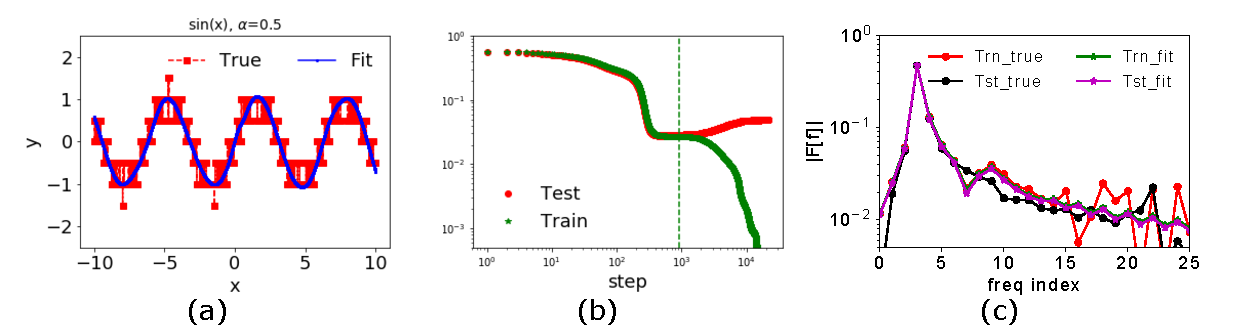
\includegraphics[width=0.98\linewidth]{figures/fprinciple/Fig3.pdf}
    \caption{图(a):使用DNN训练有噪声的正弦函数。图(b):损失函数分别在训练集测试集上的表现。图(c):训练集测试集在频率空间上的表现。}
    \label{fprinciple1}
\end{figure}


下面再举个更定量的例子,用来说明当正弦函数与其他高频函数叠加时,DNN会优先学习到更低频的部分,即正弦函数部分。从图\ref{fig:fpthree}可以看出,当DNN学习由函数$\sin (x)+\sin (5x)$生成的数据时,当epoch等于18000,神经网络可以学习处这个函数的大致趋势,并能较好的学习到$\sin (x)$的部分。只有当epoch继续增加,DNN才能学好这个函数各种高频的细节。
\begin{figure}[htbp!]
    \centering
    \subfigure[epoch:0]{
      \label{fig:subfig:onefunction} 
      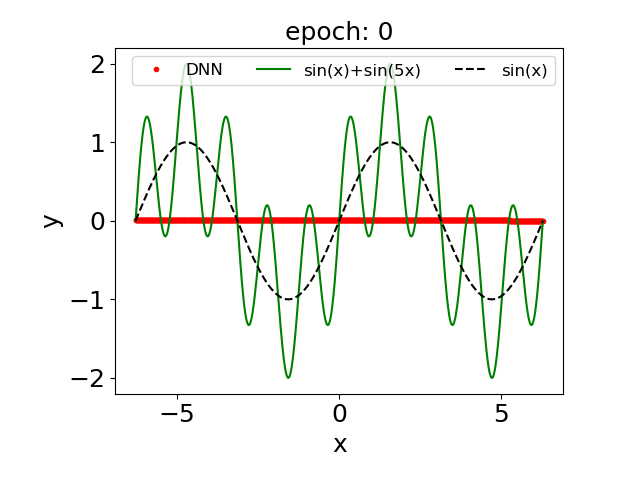
\includegraphics[scale=0.31]{figures/fprinciple/211210091512/ytestlow0.png}}
    % \hspace{0.5in} % 两图片之间的距离
    \subfigure[epoch:18000]{
      \label{fig:subfig:twofunction} 
      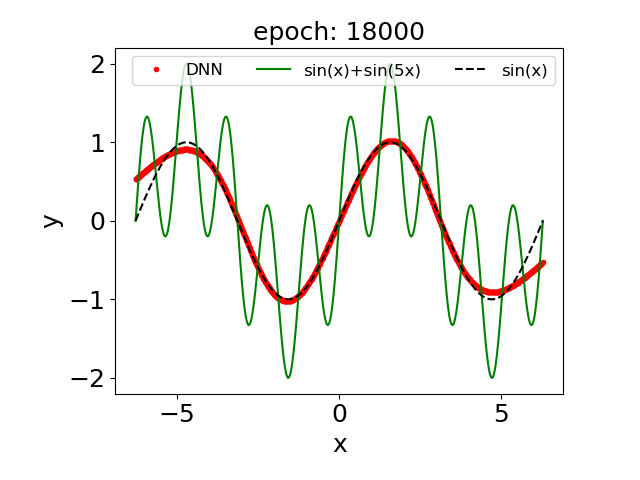
\includegraphics[scale=0.31]{figures/fprinciple/211210091512/ytestlow18000.png}}
      \subfigure[epoch:50000]{
      \label{fig:subfig:threefunction} 
      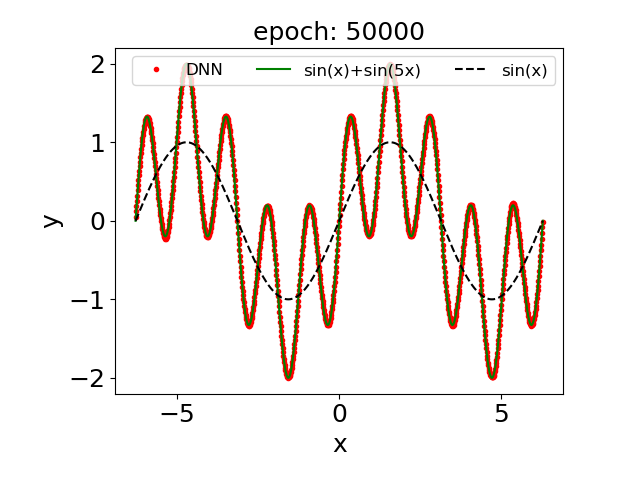
\includegraphics[scale=0.31]{figures/fprinciple/211210091512/ytestlow50000.png}}
    \caption{DNN学习函数$\sin (x)+\sin (5x)$,学习结果随epoch的变化,并与$\sin (x)$进行比较}
    \label{fig:fpthree}
  \end{figure}

从上面两个例子可以看出DNN确实可以先学习到低频部分,再学习到低频部分。那么,在学习中子共振的数据时,是不是只要我的epoch足够大,就一定能学好呢?答案显然不是,否则也没有发明PPSDNN算法的必要了。下面使用一个具体例子说明当频率稍微大一点时,传统DNN要学习好他们就必须付出极高的代价。在数值分析中,当插值函数的次数比较大时,会出现龙格现象。当使用DNN训练这类数据时,当参数数量和插值次数相仿时,就需要花费无穷大的epoch去训练他们,如图\ref{fig:fpfour}所示。有了f-principle的指导,在DNN中就不用再担龙格现象,并可以通过训练提前停止来避免过拟合。
\begin{figure}[htbp!]
    \centering
    \subfigure[epoch:250]{
      \label{onefunction} 
      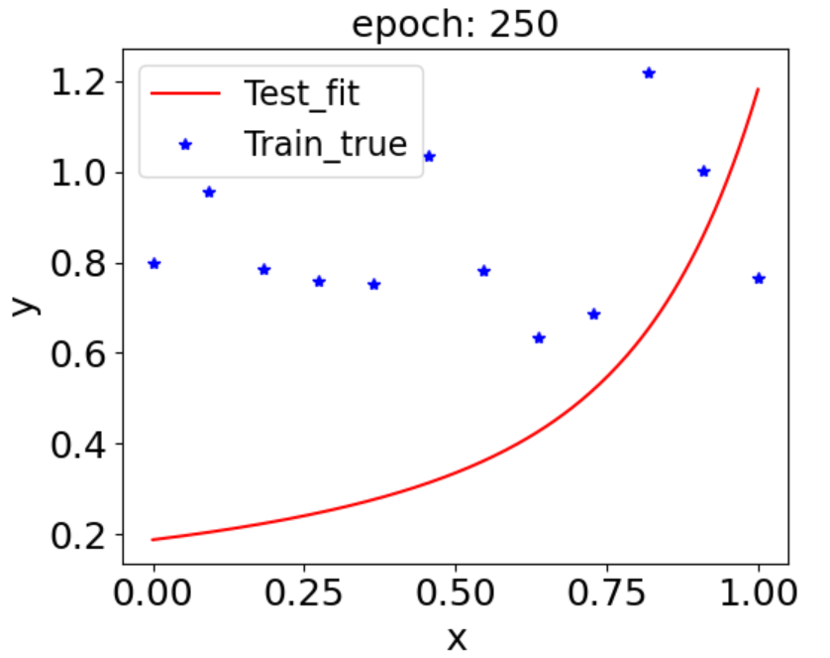
\includegraphics[scale=0.18]{figures/fprinciple/runge/e250.png}}
    % \hspace{0.5in} % 两图片之间的距离
    \subfigure[epoch:17500]{
      \label{twofunction} 
      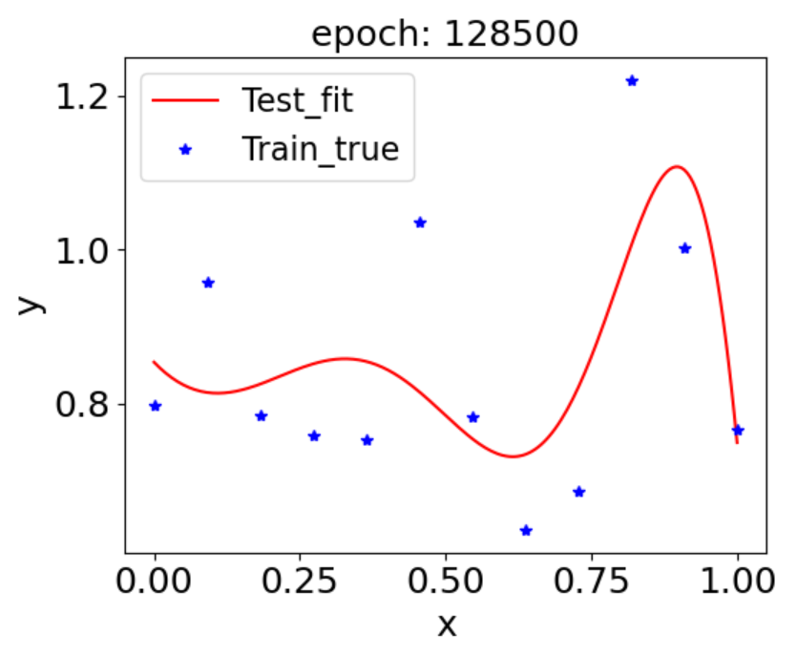
\includegraphics[scale=0.18]{figures/fprinciple/runge/e128500.png}}
      \subfigure[epoch:60750]{
      \label{threefunction} 
      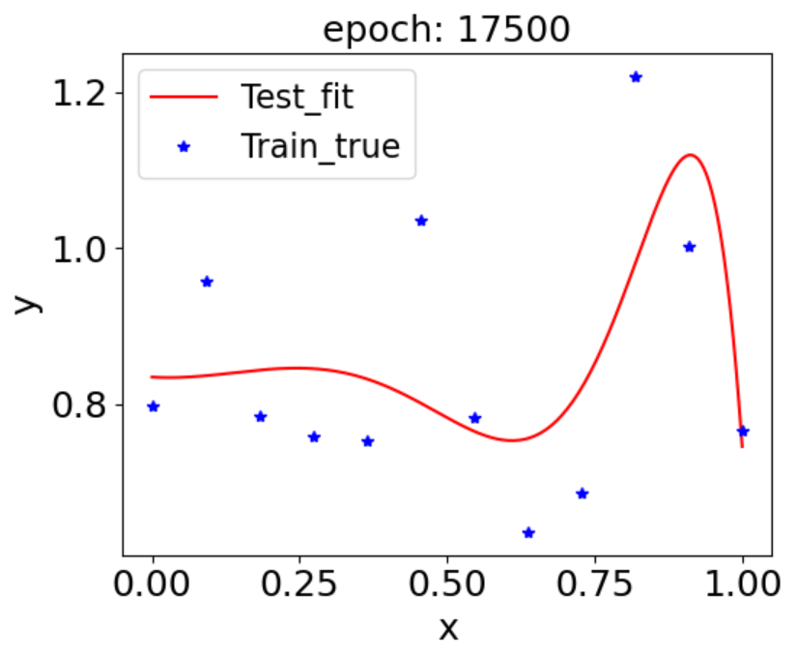
\includegraphics[scale=0.18]{figures/fprinciple/runge/e17500.png}}
      \subfigure[epoch:628500]{
      \label{fourfunction} 
      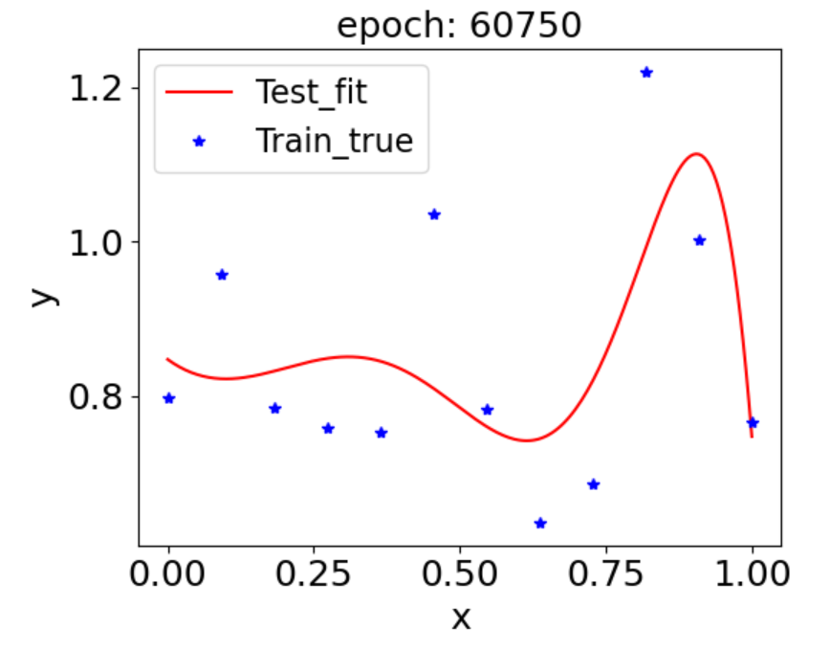
\includegraphics[scale=0.18]{figures/fprinciple/runge/e60750.png}}
    \caption{使用梯度下降学习11阶插值函数}
    \label{fig:fpfour}
  \end{figure}


f-principle 可以帮助我们理解DNN在不同问题上的优势和局限性,以及如何利用它们来设计更有效的算法。例如,在偏微分方程的数值求解中\cite{cai1996adaptive},可以结合DNN和传统迭代方法,先利用DNN快速收敛低频部分,再用传统迭代方法细化高频部分。

在中子共振核反应中,由于共振峰的存在,并根据第一章中的分析,在有限的高频共振能区中含有900多个共振峰,DNN并不能直接很好地应用于中子共振核反应的研究中。


使用DNN训练$^{235}\text{U}(n,f)$评价库数据,如图\ref{u235fp}所示,发现DNN只能较好的学习1/v能区和不可分辨能区的数据,对共振区的数据只能学习大致趋势,无法学到共振细节。为了验证DNN的训练效果不会随着epoch显著增加,可以画出损失函数的变化趋势,如图\ref{fig:u235fploss}所示,可以看出loss值在一定epoch之后不会再发生显著下降,即神经网络的学习效果不会再变好了。
\begin{figure}[htbp!]
    \centering
    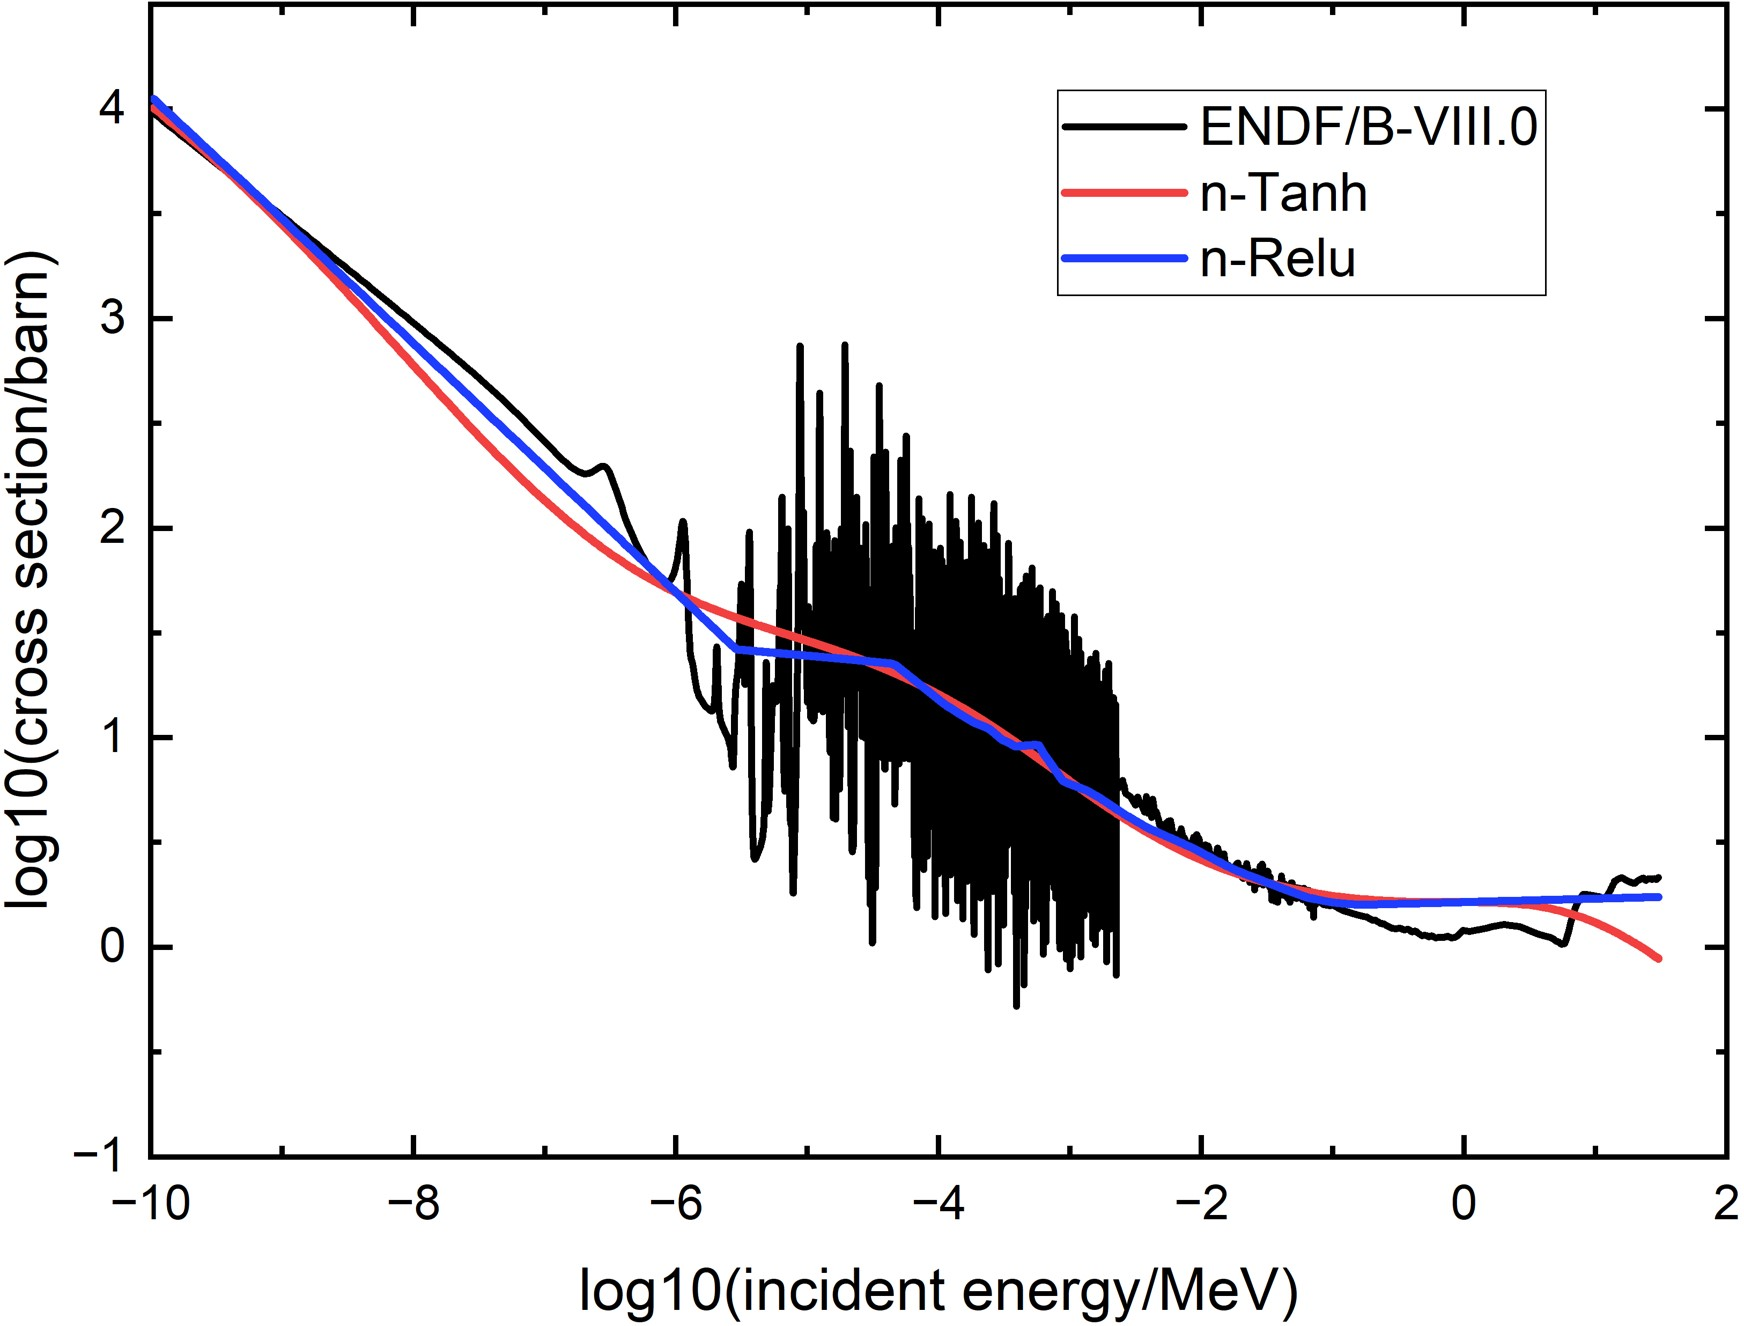
\includegraphics[width=0.76\linewidth]{figures/fprinciple/u235fp.jpg}
    \caption{使用tanh和relu激活函数分别对ENDF/B-VIII.0中$^{235}\text{U}(n,f)$反应截面进行学习}
    \label{u235fp}
\end{figure}
\begin{figure}[htbp!]
    \centering
    \subfigure[epoch:250]{
      \label{onefunu235relulossction} 
      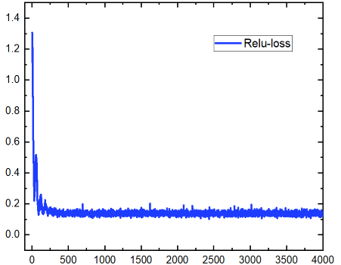
\includegraphics[scale=0.7]{figures/fprinciple/u235reluloss.png}}
    \hspace{0.5in} % 两图片之间的距离
    \subfigure[epoch:17500]{
      \label{u235tanhloss} 
      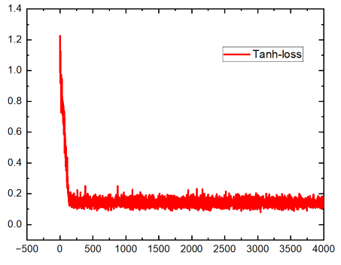
\includegraphics[scale=0.7]{figures/fprinciple/u235tanhloss.png}}
    \caption{不同激活函数下DNN的损失函数}
    \label{fig:u235fploss}
  \end{figure}


为解决DNN难以学习高频数据这个问题。本文中采用平行相移深度神经网
络模型\cite{cai2019phasednn}(Parallel Phase Shift Deep Neural Network,PPSDNN)。

\section{平行相移深度神经网络模型}

\subsection{模型及算法简介}
PPSDNN可以在训练过程中实现对函数的收敛,即同时逼近目标函数的低频和高频成分。PPSDNN利用了一个事实,即常见的DNN在训练时先收敛于低频范围,因此,它构造了一系列大小适中的DNN,并通过在频域上对训练数据进行相移操作,使得每个DNN能够逼近目标函数在特定范围内的高频内容。由于相移的作用,每个DNN都能够像在低频范围一样快速收敛。因此,PPSDNN能够将高频学习转化为低频学习,从而实现对函数的全部频域空间均匀学习和自适应训练。\cite{daubechies1992ten}
算法的大致思想是利用神经网络在训练过程中对低频成分的快速收敛,
通过相移技术将目标函数的高频成分转换为低频成分,然后用一系列并行的神经网络来近似不同频率范围的函数,
最后将这些神经网络的输出相加,从而得到目标函数的近似。

PPSDNN算法的基本思路如下:首先,将$f(x)$分解成各个频段函数的叠加。
\begin{equation}
f(x)=%
%TCIMACRO{\dsum \limits_{j=0}^{m}}%
%BeginExpansion
{\displaystyle\sum\limits_{j=0}^{m}}
%EndExpansion
f_{j}(x), \label{x-decomp}%
\end{equation}
其中,
\[
f_{j}(x)=\mathcal{F}^{-1}[\widehat{f_{j}}](x).
\]
谱区间为$[\omega _{j-1},\omega _{j+1}]$
设对于低频项,频域$k\in [-K_0,k_0]$,普通DNN方法可以给出很好的近似。
对于高频项,通过相移(phase shift)$r_{j}^{\text{shift}}(x_{i})=e^{i\omega_{j}x_{i}}r_{j}(x_{i})$,把高频数据转换成$[-K_0,k_0]$上的低频数据,进而使用DNN训练。将训练得到的结果再通过phase shift还原到高频部分。最后将训练的到的所有结果加起来就是总的训练结果。

PPSDNN算法可按如下几个模块逐步实现:
\begin{enumerate}
    \item 傅里叶变换和与尼奎斯特采样定理\cite{vaidyanathan2001generalizations}
    \item 单位分解定理(POU)
    \item B-样条函数
    \item 相移在频域空间中的实现
\end{enumerate}
\subsection{傅里叶变换与尼奎斯特采样定理}
傅里叶变换是把一个函数或一些离散数据从时域空间转换到频域空间,傅里叶逆变换则是从频域空间转换到时域空间\cite{xu2018understanding}。先考虑连续傅里叶变换(CFT)和连续傅里叶逆变换(ICFT),其公式为
    \begin{equation}
\mathcal{F}[g(x)](\xi)=\int_{-\infty}^{\infty} g(x) \mathrm{e}^{-2 \pi \mathrm{i} \xi x} \mathrm{~d} x, \quad \mathcal{F}^{-1}[\hat{g}(\xi)](x)=\int_{-\infty}^{\infty} \hat{g}(\xi) \mathrm{e}^{2 \pi \mathrm{i} \xi x} \mathrm{~d} \xi
\end{equation}
再考虑离散时域空间上的傅里叶变换(DTFT)及其逆变换
\begin{equation}
\begin{aligned}
& \mathcal{F}_{D T F T, \Delta}[g(x)](\xi)=\hat{g}_{D T F T}(\xi)=\sum_{j=-\infty}^{\infty} g(j \Delta) \mathrm{e}^{-2 \pi \mathrm{i} \xi j \Delta} \\
& \mathcal{F}_{D T F T, \Delta}^{-1}[\hat{g}(\xi)](j)=\Delta \cdot \int_{-\frac{1}{2 \Delta}}^{\frac{1}{2 \Delta}} \hat{g}_{D T F T}(\xi) \mathrm{e}^{2 \pi \mathrm{i} \xi j \Delta} \mathrm{d} \xi
\end{aligned}
\end{equation}
由于客观世界的数据往往是连续分布的,而我们认识的世界往往是通过离散的采样得到的数据。于是我们要尽可能在最大限度保留真实世界信息的情况下把CFT向DTFT转换。下面是转换公式的推导
\begin{equation}
\begin{aligned}
& \mathcal{F}_{D T F T, \Delta}[g(x)](\xi)=\sum_{j=-\infty}^{\infty} g(j \Delta) \mathrm{e}^{-2 \pi \mathrm{i} \xi j \Delta} \\
& =\sum_{j=-\infty}^{\infty} \int_{-\infty}^{\infty} \hat{g}\left(\xi^{\prime}\right) \mathrm{e}^{2 \pi \mathrm{i} \xi^{\prime} j \Delta} \mathrm{d} \xi^{\prime} \mathrm{e}^{-2 \pi \mathrm{i} \xi j \Delta} \\
& =\sum_{j=-\infty}^{\infty} \sum_{M=-\infty}^{\infty} \int_{\frac{M}{\Delta}-\frac{1}{2 \Delta}}^{\frac{M}{\Delta}+\frac{1}{2 \Delta}} \hat{g}\left(\xi^{\prime}\right) \mathrm{e}^{2 \pi \mathrm{i} \xi^{\prime} j \Delta} \mathrm{d} \xi^{\prime} \mathrm{e}^{-2 \pi \mathrm{i} \xi j \Delta} \\
& =\sum_{j=-\infty}^{\infty} \sum_{M=-\infty}^{\infty} \int_{-\frac{1}{2 \Delta}}^{\frac{1}{2 \Delta}} \hat{g}\left(\xi^{\prime}+\frac{M}{\Delta}\right) \mathrm{e}^{2 \pi \mathrm{i} \xi^{\prime} j \Delta} \mathrm{d} \xi^{\prime} \mathrm{e}^{-2 \pi \mathrm{i} \xi j \Delta} \\
&
\end{aligned}
\end{equation}
定义$\hat{h}\left(\xi^{\prime}\right)=\hat{g}\left(\xi^{\prime}+\frac{M}{\Delta}\right)$,得
\begin{equation}
\mathcal{F}_{D T F T, \Delta}[g(x)](\xi)=\frac{1}{\Delta} \sum_{M=-\infty}^{\infty} \sum_{j=-\infty}^{\infty}\left(\Delta \int_{-\frac{1}{2 \Delta}}^{\frac{1}{2 \Delta}} \hat{h}\left(\xi^{\prime}\right) \mathrm{e}^{2 \pi \mathrm{i} \xi^{\prime} j \Delta} \mathrm{d} \xi^{\prime}\right) \mathrm{e}^{-2 \pi \mathrm{i} \xi j \Delta}
\end{equation}
通过逆DTFT得
\begin{equation}
    \mathcal{F}_{DTFT,\Delta}[g(x)](\xi)=\dfrac{1}{\Delta}\sum\limits_{M=-\infty}^\infty\sum\limits_{j=-\infty}^\infty h(j\Delta)\mathrm{e}^{-2\pi i\xi j\Delta}.
\end{equation}
再通过DTFT得
\begin{equation}
    \begin{aligned}\mathcal{F}_{DTFT,\Delta}[g(x)](\xi)&=\frac{1}{\Delta}\sum_{M=-\infty}^\infty\bar{h}(\xi)\\ &=\frac{1}{\Delta}\sum_{M=-\infty}^\infty\hat{g}(\xi+\frac{M}{\Delta}).\end{aligned}
\end{equation}
在上式中,左边是离散时间中的采样,右边代表真是信号。其中,左边的$\xi \in [-\frac{1}{2\Delta },\frac{1}{2\Delta }  ]$。于是,可以得到尼奎斯特采样定理\cite{benedetto2001modern}。
\begin{thm}
一个有限带宽的连续信号可以被采样并且可以从它的采样中完美重构的条件为:采样频率大于真实频率的两倍。
\end{thm}
有了尼奎斯特采样定理,我们就能知道至少需要多少实验数据点才能学好中子共振截面的数据。

\subsection{单位分解定理}
在数学上,任意流形都能够表示成足够大的n维空间$\mathbb{R}^n$中某个曲面形式,而这可以用单位分解定理(Partition of Unity,POU)\cite{卓里奇2019数学分析}阐明。

\begin{thm}
设M是$C^{(k)}$光滑类的流形,X是M的子集。如果函数组$E= \{e_{\alpha},\alpha \in A\}$由$e_{\alpha} = C^{(k)}(M,\mathbb{R})$组成,且满足:

在X上$\sum_{e_{\alpha }\in E}^{}e_{\alpha }(x)\equiv 1 $。

那么,我们就说该函数组是集合X上的k阶光滑单位分解。
\end{thm}
在PPSDNN中,我们首先要将一个含有高频部分的目标函数f(x)通过傅里叶变换高频谱函数$\hat{f}(k)$,
再通过phase shift将频谱转换到$[-K_0,K_0]$的范围。下面考虑
$\widehat{f}(k)$上的支撑集,因为$\text{supp}\widehat{f}(k)=\{k \in \mathbb{R}|\widehat{f}(k)\ne 0\}$,
所以对给定的$\Delta k$,可以设$\widehat{f}(k)$上的支撑集为$\text{supp}\widehat{f}(k)\subset\lbrack-m\Delta k,m\Delta k].$。再将区间$[-m\Delta k,m\Delta k]$格点化,令$\omega _j = j \Delta k$,其中,$j = -m,...-1,0,1,...m$。下面考虑在区间$[-m\Delta k,m\Delta k]$上进行单位分解
\begin{equation}
1=%
%TCIMACRO{\dsum \limits_{j=0}^{m}}%
%BeginExpansion
{\displaystyle\sum\limits_{j=-m}^{m-1}}
%EndExpansion
\phi_{j}(k),\text{ }k\in\lbrack -m\Delta k,m\Delta k].\label{pou}%
\end{equation}

下面举几个满足单位分解定理的例子。
满足单位分解最简单的函数为$\phi _{j}(k)$:
\begin{equation}\label{eq:phij}
  \phi_j(k)=\phi(\frac{k-\omega_{j}}{\Delta k}) = \phi (\frac{k}{\Delta k}-j),
\end{equation}
其中,$\phi (k)$是区间$[-1,1)$上的特征函数,特征函数的形式为
\begin{equation}
    \phi (k) = \chi _{[0,1)}(k)= 
  \left\{\begin{matrix} 
  1,k \in[0,1)\\ 
  0,otherwise \\ 
\end{matrix}\right.  
\end{equation}
则对$\phi _j(k)$而言,$0\le \frac{k-\omega _j}{\Delta k}<1 $时,即$j\Delta k\le k<(j+1)\Delta k$时为1,其余区间为0,即
\begin{equation}
    \phi _j(k)= \left\{\begin{matrix} 
  1,k \in[j\Delta k,(j+1)\Delta k)\\ 
  0,otherwise \\ 
\end{matrix}\right.
\end{equation}
这样的2m个函数$\phi_{-m}(k),\phi_{-m+1}(k),...\phi_{0}(k),...\phi_{m-2}(k),\phi_{m-1}(k),$
对应的值为1的非零区间为$[-m\Delta k,(-m+1)\Delta k),[-(m+1)\Delta k,(-m+2)\Delta k),...,[(m-2)\Delta k,(m-1)\Delta k),[(m-2)\Delta k,(m-1)\Delta k)$。因此,当$-m\Delta k\le  k\le m\Delta k$时,必落在某个区间,使某个$\phi _j(k)=1$,其余的$\phi _j(k)=0$,即$\sum_{j=-m }^{m-1}\phi_j(k) = 1$。因此$\phi_j(k)$满足单位分解定理(POU)。下面计算$\phi (k) = \chi _{[0,1)}(k)$的逆傅里叶变换,我们用符号$\vee$表示。
\begin{equation}\label{eq:invfphi}
  \phi^{\vee}(x) = \frac{1}{\sqrt{2\pi} } \int_{0}^{1} dke^{ikx}=\frac{e^{\frac{ix}{2}(e^{\frac{ix}{2} }-e^{-\frac{ix}{2} }) }}{ix\sqrt{2\pi}}
  = \frac{1}{\sqrt{2\pi}}e^{i\frac{x}{2}}\frac{\sin x/2}{x/2}.
\end{equation}

 虽然特征函数可以构造出满足单位分解的函数,但特征函数是分段函数,且不够光滑。下面我们使用B-样条函数构造满足单位分解的函数,这样的函数满足连续且光滑的条件。



\subsection{B-样条函数}
B-样条函数\cite{prochazkova2005derivative}是基于特征函数迭代递推得到的,它和特征函数相比具有更连续更光滑的性质。采用如下卷积迭代的方式可以定义B-样条函数
\begin{equation}
    \left\{\begin{matrix} 
&B_{1}(k)=\chi_{\lbrack0,1)}(k),\\
&B_{m}(k)=B_{m-1}(k)\ast\chi_{\lbrack0,1)}(k),m=2,\cdots.\label{b-spline}%
\end{matrix}\right. 
\end{equation}
这种递推关系式也可以写成
\begin{equation}
    B_{m}(k)=\underbrace{B_1(k) * B_{1}(k) * \cdots * B_{1}(k)}_{m \text{个}}
\end{equation}
其中$*$代表卷积,即$(f * g)(t) \stackrel{\text { def }}{=} \int_{\mathbb{R}^{n}} f(\tau) g(t-\tau) d \tau$
可以用归纳法证明
\begin{equation}
    supp B_{m}(k)=[0,m)
\end{equation}
下面,分别举m=2和m=3的例子来说明B-样条函数的支撑集以及它的连续性和光滑性。

当m=2时
\begin{equation*}
    B_{2}(k)=B_{1}(k)\star B_{1}(k)=\int_{-\infty}^{\infty}B_{1}(k-\lambda)B_{1}(\lambda)d\lambda=
\int_{0}^{1}B_{1}(k-\lambda)d\lambda
\end{equation*}
其中
\begin{equation*}
    \left\{\begin{matrix} 
0 \le \lambda <1,\\
0\le k-\lambda <1
\end{matrix}\right. 
\Rightarrow 0\le k <2
\end{equation*}
于是不难看出
\begin{equation}
    supp B_2(k)=[0,2)
\end{equation}
通过积分,不难得出
\begin{equation}
B_2(k)=
    \left\{\begin{matrix} 
k,0\le k<1\\
2-k,1\le k<2\\
0,otherwise
\end{matrix}\right. 
\end{equation}
可以看出,$B_2(k)$虽然连续,但不光滑。如图\ref{B2}
\begin{figure}[htbp]
    \centering
    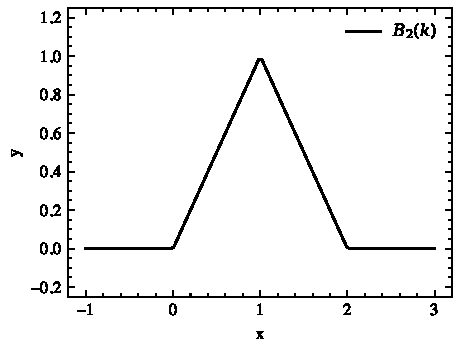
\includegraphics[width=0.76\linewidth]{figures/B-splin/B2.pdf}
    \caption{2阶B样条函数}
    \label{B2}
\end{figure}

当m=3时,同理可得
\begin{equation*}
    B_{3}(k)=B_{2}(k)\star B_{1}(k)=\int_{-\infty}^{\infty}B_{2}(k-\lambda)B_{1}(\lambda)d\lambda=
\int_{0}^{1}B_{2}(k-\lambda)d\lambda
\end{equation*}
且不难看出
\begin{equation}
    supp B_3(k)=[0,3)
\end{equation}
通过积分,不难得出
\begin{equation}
B_3(k)=
    \left\{\begin{matrix} 
\frac{1}{2}k^2 ,0\le k<1\\
\frac{1}{2}+(k-1)-(k-1)^2 ,1\le k<2\\
\frac{1}{2}-(k-2)+\frac{1}{2} (k-2)^2 ,2\le k<3\\
0,otherwise
\end{matrix}\right. 
\end{equation}
此时,在k=1和k=2处,$B_3(k)$不仅连续,而且光滑(一阶导数连续)。如图\ref{B3}
\begin{figure}[htbp]
    \centering
    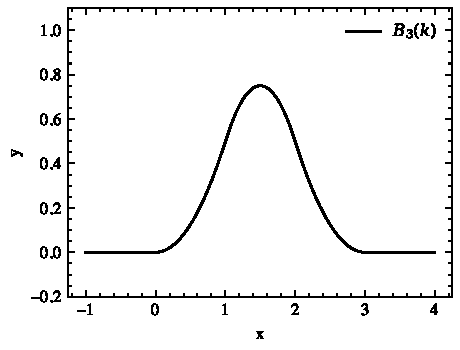
\includegraphics[width=0.76\linewidth]{figures/B-splin/B3.pdf}
    \caption{3阶B样条函数}
    \label{B3}
\end{figure}

于是,可以整理出B-样条函数的诸多性质,如
\begin{enumerate}
    \item $\text{supp} B_m(k)=[0,m)$
    
    证明:采用归纳法。

    在上文中,我们通过计算m=1,m=2,m=3给出了具体几个常用特例的证明。下面,采用数学归纳法给出普式的m的证明。

    设$\text{supp} B_m(k)=[0,m)$,则
    \begin{equation*}
    B_{m+1}(k)=B_{m}(k)\star B_{1}(k)=\int_{-\infty}^{\infty}B_{m}(k-\lambda)B_{1}(\lambda)d\lambda=
\int_{0}^{1}B_{m}(k-\lambda)d\lambda
\end{equation*}
其中
\begin{equation*}
    \left\{\begin{matrix} 
0 \le \lambda <1,\\
0\le k-\lambda <m
\end{matrix}\right. 
\Rightarrow 0\le k <m+1
\end{equation*}
于是,$\text{supp} B_m(k)=[0,m)$,证毕。
    \item $B_m(k)$的逆傅里叶变换
    
    通过卷积定理:
    \begin{equation}
        \left\{\begin{matrix} 
& \mathcal{F} [f(x)*g(x)]= \hat{f}(k)\hat{g}(k)  \\
& \mathcal{F}[f(x)g(x)] = \hat{f}(k)*\hat{g}(k)\Rightarrow f(x)g(x) = \mathcal{F}^{-1}[\hat{f}(k)*\hat{g}(k)] \\
\end{matrix}\right. 
    \end{equation}
其中,为了符号书写方便,把傅里叶逆变换定义为$\mathcal{F[\cdot ]}$。

这样,$B_m(k)$的逆傅里叶变换,记为$B_m^{\vee}(k)$,有
\begin{align}
B_{m}^{\vee}(x)  &  =\left(  B_{1}^{\vee}(x)\right)  ^{m}=\left(  \frac
{1}{\sqrt{2\pi}}e^{i\frac{x}{2}}\frac{\sin\frac{x}{2}}{\frac{x}{2}}\right)
^{m}\nonumber\\
&  =\frac{e^{i\frac{mx}{2}}}{\left(  2\pi\right)  ^{m/2}}\left(  \frac
{\sin\frac{x}{2}}{\frac{x}{2}}\right)  ^{m}.
\end{align}
\end{enumerate}
下面将在“相移在频域空间中的实现”部分介绍如何使用B-样条函数构造满足单位分解的函数。


\subsection{相移在频域空间中的实现}
我们以四次B-样条函数为例,构造满足单位分解的函数。首先,令$\phi(k)=B_{4}(k+2)$,接着构造
\begin{equation}
    \phi_j(k)=\phi(k/\Delta k-j)=B_4(\frac{k}{\Delta k}+2-j)
\end{equation}

可以证明,该函数满足单位分解。将$\phi_j(k)$做傅里叶逆变换,得到频率选择函数(frequency selection kernel),为了得到$\phi_{j}^{\vee}(x)$,我们先求$\phi^{\vee}(x)$,得
\begin{equation}
    \begin{aligned} 
        &\phi^{\vee}(x) =\frac{1}{\sqrt[]{2\pi } }\int_{\mathcal{R} }^{}  B_4(k+2)e^{ikx}dk \\
      &\overset{令k+2=k'}{=} \frac{1}{\sqrt[]{2\pi } }\int_{\mathcal{R} }^{}dk'B_4(k')e^{ik'x}e^{-2ix}\\
      &=B_4^{\vee } (x)e^{-2ix}=\frac{1}{(2\pi)^2}(\frac{\sin{x/2}}{x/2})^4
      \end{aligned}
\end{equation}
下面计算$\phi_j(k)$的傅里叶逆变换,的
\begin{equation}
    \begin{aligned} 
        & \phi_{j}^{\vee}(x)=\frac{1}{\sqrt[]{2\pi } }\int_{\mathcal{R} }^{}dk\phi(\frac{k}{\Delta k}-j )e^{ikx}  \\
       &\overset{k'=k/\Delta k}{=}\frac{1}{\sqrt[]{2\pi } }\int_{\mathcal{R} }^{}  (\Delta k)dk'\phi (k'-j)e^{ik'\Delta kx}  \\
       &\overset{k''=k'-j}{=}\frac{1}{\sqrt[]{2\pi } }\int_{\mathcal{R} }^{}  (\Delta k)dk''\phi (k'')e^{i(k''+j)\Delta kx}\\
       &=\Delta ke^{-ij\Delta kx}\phi^{\vee}(\Delta kx)=K_0e^{-ijK_{0}x}%
       \phi^{\vee}(K_{0}x),
       \end{aligned},
\end{equation}
下面求$\phi_{j}(k)$的支撑集。由前面的定义和结论,显然,有$supp\phi _j(k)=supp\mathcal{F}[\phi_{j}^{\vee}(x)]$。于是,根据$0\le \frac{k}{\Delta k}+2-j<4$得,$\omega_{j-2}\le k<\omega_{j+2}$,即
\begin{equation}
    supp\mathcal{F}[\phi_{j}^{\vee}(x)]\subset\lbrack\omega_{j-2}, \omega_{j+2}].
\end{equation}

同样,可以证明B-样条函数满足单位分解性质。
前面假设了低频空间为$k\in [-m\Delta k,\Delta k]$,通过移项得$-m\le \frac{k}{\Delta k}\le m$。又$0\le \frac{k}{\Delta k}+2-j<4$,移项得$-2+\frac{k}{\Delta k}<j\le 2+\frac{k}{\Delta k}$。不难得出
\begin{equation*}
    -m-2<j\le m+2
\end{equation*}
因此,j实际的范围是$j = -m-1,-m,...,0,...,m+1,m+2$。
因此,可以证明$\phi_{j}(k)$满足单位分解。
\begin{equation}\label{eq:sum1C4}
  \sum_{j=-m-1}^{m+2}\phi_j(k) = 1 ,\quad \forall k\in [-m\Delta k, m\Delta k].
\end{equation}
在实际我们选择POU函数时,对于$\sum_{j}^{}\phi_j(k) = 1$,j的具体范围取决于:

    1) k的范围;
    2) 样条函数的选取;
    3) 样条函数的平移量。


然后,在POU的基础上,我们对想要分解的函数f(x)做傅里叶展开(傅里叶逆变换),即
\begin{equation}
    f(x) = \frac{1}{\sqrt{2\pi}}\int_{\mathcal{R} }^{}dk\hat{f}(x)e^{ikx}  \label{Ff}
\end{equation}
其中,$\hat{f}(k)$可以利用POU的性质分解为
\begin{equation}
\widehat{f}(k)=%
%TCIMACRO{\dsum \limits_{j=0}^{m}}%
%BeginExpansion
{\displaystyle\sum\limits_{j=-m}^{m-1}}
%EndExpansion
\phi_{j}(k)\widehat{f}(k)\triangleq%
%TCIMACRO{\dsum \limits_{j=0}^{m}}%
%BeginExpansion
{\displaystyle\sum\limits_{j=-m}^{m-1}}
%EndExpansion
\widehat{f_{j}}(k). \label{k-decomp}%
\end{equation}
相应的,把\ref{k-decomp}式代入\ref{Ff}式,可以在时域空间里将f(x)做分解
\begin{equation}
f(x)=%
%TCIMACRO{\dsum \limits_{j=0}^{m}}%
%BeginExpansion
{\displaystyle\sum\limits_{j=0}^{m}}
%EndExpansion
f_{j}(x), \label{x-decomp}%
\end{equation}
其中,
\[
f_{j}(x)=\mathcal{F}^{-1}[\widehat{f_{j}}](x).
\]
根据POU,
\begin{equation*}
    f_{j}(x) = \frac{1}{\sqrt{2\pi}}\int_{\omega _j }^{\omega_{j+1}}dk\hat{f_j}(k)e^{ikx}=\\
    \frac{1}{\sqrt{2\pi}}\int_{\omega _j }^{\omega_{j+1}}dk\phi_j(k)\hat{f}(k)e^{ikx}=\mathcal{F}^{-1}[\phi_j \hat{f}]
\end{equation*}
由卷积定理,$\mathcal{F}[f(x)*g(x)] = \hat{f}(k)\hat{g}(k)$,即$f(x)*g(x) = \mathcal{F}^{-1}[\hat{f}(k)\hat{g}(k)]$。
所以,
\begin{equation}
    f_j(x) = \phi_j^{\vee}(x)*f(x)=\int_{-\infty }^{\infty} \phi _j^{\vee}(x-s)f(s)ds
\end{equation}
从上式可以看出,$\phi_j^{\vee}(x)$通过卷积作用到f(x)上得到频率空间为$[\omega_j,\omega_{j+1}]=[j\Delta k,(j+1)\Delta]=[jK_0,(j+1)K_0]$的分量。$f_j(x)$在此称为频率选择函数(frequency selection kernal)。

基于频率选择函数,就可以实现平行相移。
设当函数f(x)通过傅里叶变换转换到频域空间,且$|k|<K_0$时,函数处于低频,DNN可以很好的训练f(x)的低频量。对f(x)的高频量$f_j(x)$,我们可以通过乘一个相移因子,将其转换到$|k|<K_0$的区域,具体形式为:
\begin{equation}
    f_j^{\text{shift}}(x) = e^{i\omega_jx}f_j(x)
\end{equation}
下面分析$f_j^{\text{shift}}(x)$的频率范围,这里的推导需要用到$\delta$函数的性质。
\begin{equation}
    f_j^{\text{shift}}(k) = \hat{f}_j(k-\omega_j)
\end{equation}
如果$f_j(k)$的支撑集为$[\omega_j,\omega_{j+1}]$,则$supp[f_j^{\text{shift}}(k)]\subset [0,K_0]$。于是,我们通过phase shift将f(x)的高频部分转换到了低频部分。于是可以将低频部分使用DNN去训练。下面介绍PPSDNN的算法流程。


\section{算法流程}
首先,给定一个要用来训练的目标函数f(x)。我们使用DNN$T_{\star}(x,\theta^{(n_{0}%
)}),x\in R,$去逼近它。
\begin{equation}
T_{\star}(x,\theta^{(n_{0})})=f_{\text{DNN}}(x)\approx f(x),\label{f1(x)}%
\end{equation}
$f_{\text{DNN}}(x)$和f(x)各自对应的低频部分可以拟合的很好,但高频部分仍然会有差距。于是定义余项$r(x)=f(x)-f_{\text{DNN}}(x)$,并规定低频区域
\begin{equation}
\left\vert \mathcal{F}[r](k)\right\vert \ll1\text{ for }\left\vert
k\right\vert <K_{0},
\end{equation}
这样,才能确保
\begin{equation}
\mathcal{F}[f](k)\approx\mathcal{F}[f_{\text{DNN}}(x)](k),\quad k\in
(-K_{0},K_{0}).\label{eq:1psdnn}%
\end{equation}

如果精确知道r(x),则$f(x) = r(x) + f_{\text{DNN}}(x)$。为尽量精确求得r(x),首先将r(x)分解,
\begin{equation}
r(x)=%
%TCIMACRO{\dsum \limits_{j=0}^{m}}%
%BeginExpansion
{\displaystyle\sum\limits_{j=0}^{m}}
%EndExpansion
r_{j}(x),
\end{equation}
其中
\begin{equation}
r_{j}(x)=\mathcal{F}^{-1}[\widehat{r_{j}}(k)]=\mathcal{F}^{-1}[\phi
_{j}(k)\widehat{r}(k)](x).\label{rj(x)}%
\end{equation}
训练数据$\{r_{j}(x_{i})\}_{i=1}^{N}$可以由\ref{rj(x)}式计算得到,在时域空间上,这些离散数据点可以通过下面的卷积公式得到
\begin{align}
r_{j}(x_{i}) &  =\phi_{j}^{\vee}\ast r(x_{i})=\int_{-\infty}^{\infty}\phi
_{j}^{\vee}(x_{i}-s)r(s)ds\nonumber\\
&  \approx\frac{2\delta}{N_{s}}%
%TCIMACRO{\dsum \limits_{x_{s}\in(x_{i}-\delta,x_{i}+\delta)}}%
%BeginExpansion
{\displaystyle\sum\limits_{x_{s}\in(x_{i}-\delta,x_{i}+\delta)}}
%EndExpansion
\phi_{j}^{\vee}(x_{i}-x_{s})r(x_{s}),\label{convol}%
\end{align}
取相应的频率选择核$r_{j}(x)$,可以将$\phi_j(x)$的频率范围,即支撑集调整到$[\omega_{j-1,}\omega_{j+1}]$。


接下来对$r_j(x)$作phase shift。
\begin{equation}
r_{j}^{\text{shift}}(x)=e^{i\omega_jx}r_j(x)=\mathcal{F}^{-1}\left[  \widehat{r_{j}}(k-\omega
_{j})\right]  (x),\label{rjshift}%
\end{equation}
则$r_{j}^{\text{shift}}(x)$的支撑集在$[-K_0,K_0]$之间。所以$r_{j}^{\text{shift}}(x)$属于低频部分,所以它可以由DNN相对精确且快速地得到。即
\begin{equation}
T_{j}(x,\theta^{(n_{0})})\ \approx r_{j}^{\text{shift}}(x),0\leq j\leq m,
\end{equation}
相应的$r_j(x)$为
\begin{equation}
r_{j}(x)\approx e^{-i\omega_{j}x}T_{j}(x,\theta^{(n_{0})}).
\end{equation}
于是
\begin{equation}
r(x)\approx%
%TCIMACRO{\dsum \limits_{j=0}^{m}}%
%BeginExpansion
{\displaystyle\sum\limits_{j=0}^{m}}
%EndExpansion
e^{-i\omega_{j}x}T_{j}(x,\theta^{(n_{0})}).
\end{equation}
最终,我们得到
\begin{equation}
f(x) \approx f_{\text{DNN}}(x)+%
%TCIMACRO{\dsum \limits_{j=0}^{m}}%
%BeginExpansion
{\displaystyle\sum\limits_{j=0}^{m}}
%EndExpansion
e^{-i\omega_{j}x}T_{j}(x,\theta^{(n_{0})}). \label{DNNupdate}%
\end{equation}
以上便是PPSDNN的全部算法。本算法可以使用python语言实现,用pytorch\cite{ketkar2021introduction}编写,算法大致流程如图\ref{ppsdnnchart}:
\begin{figure}[htbp]
    \centering
    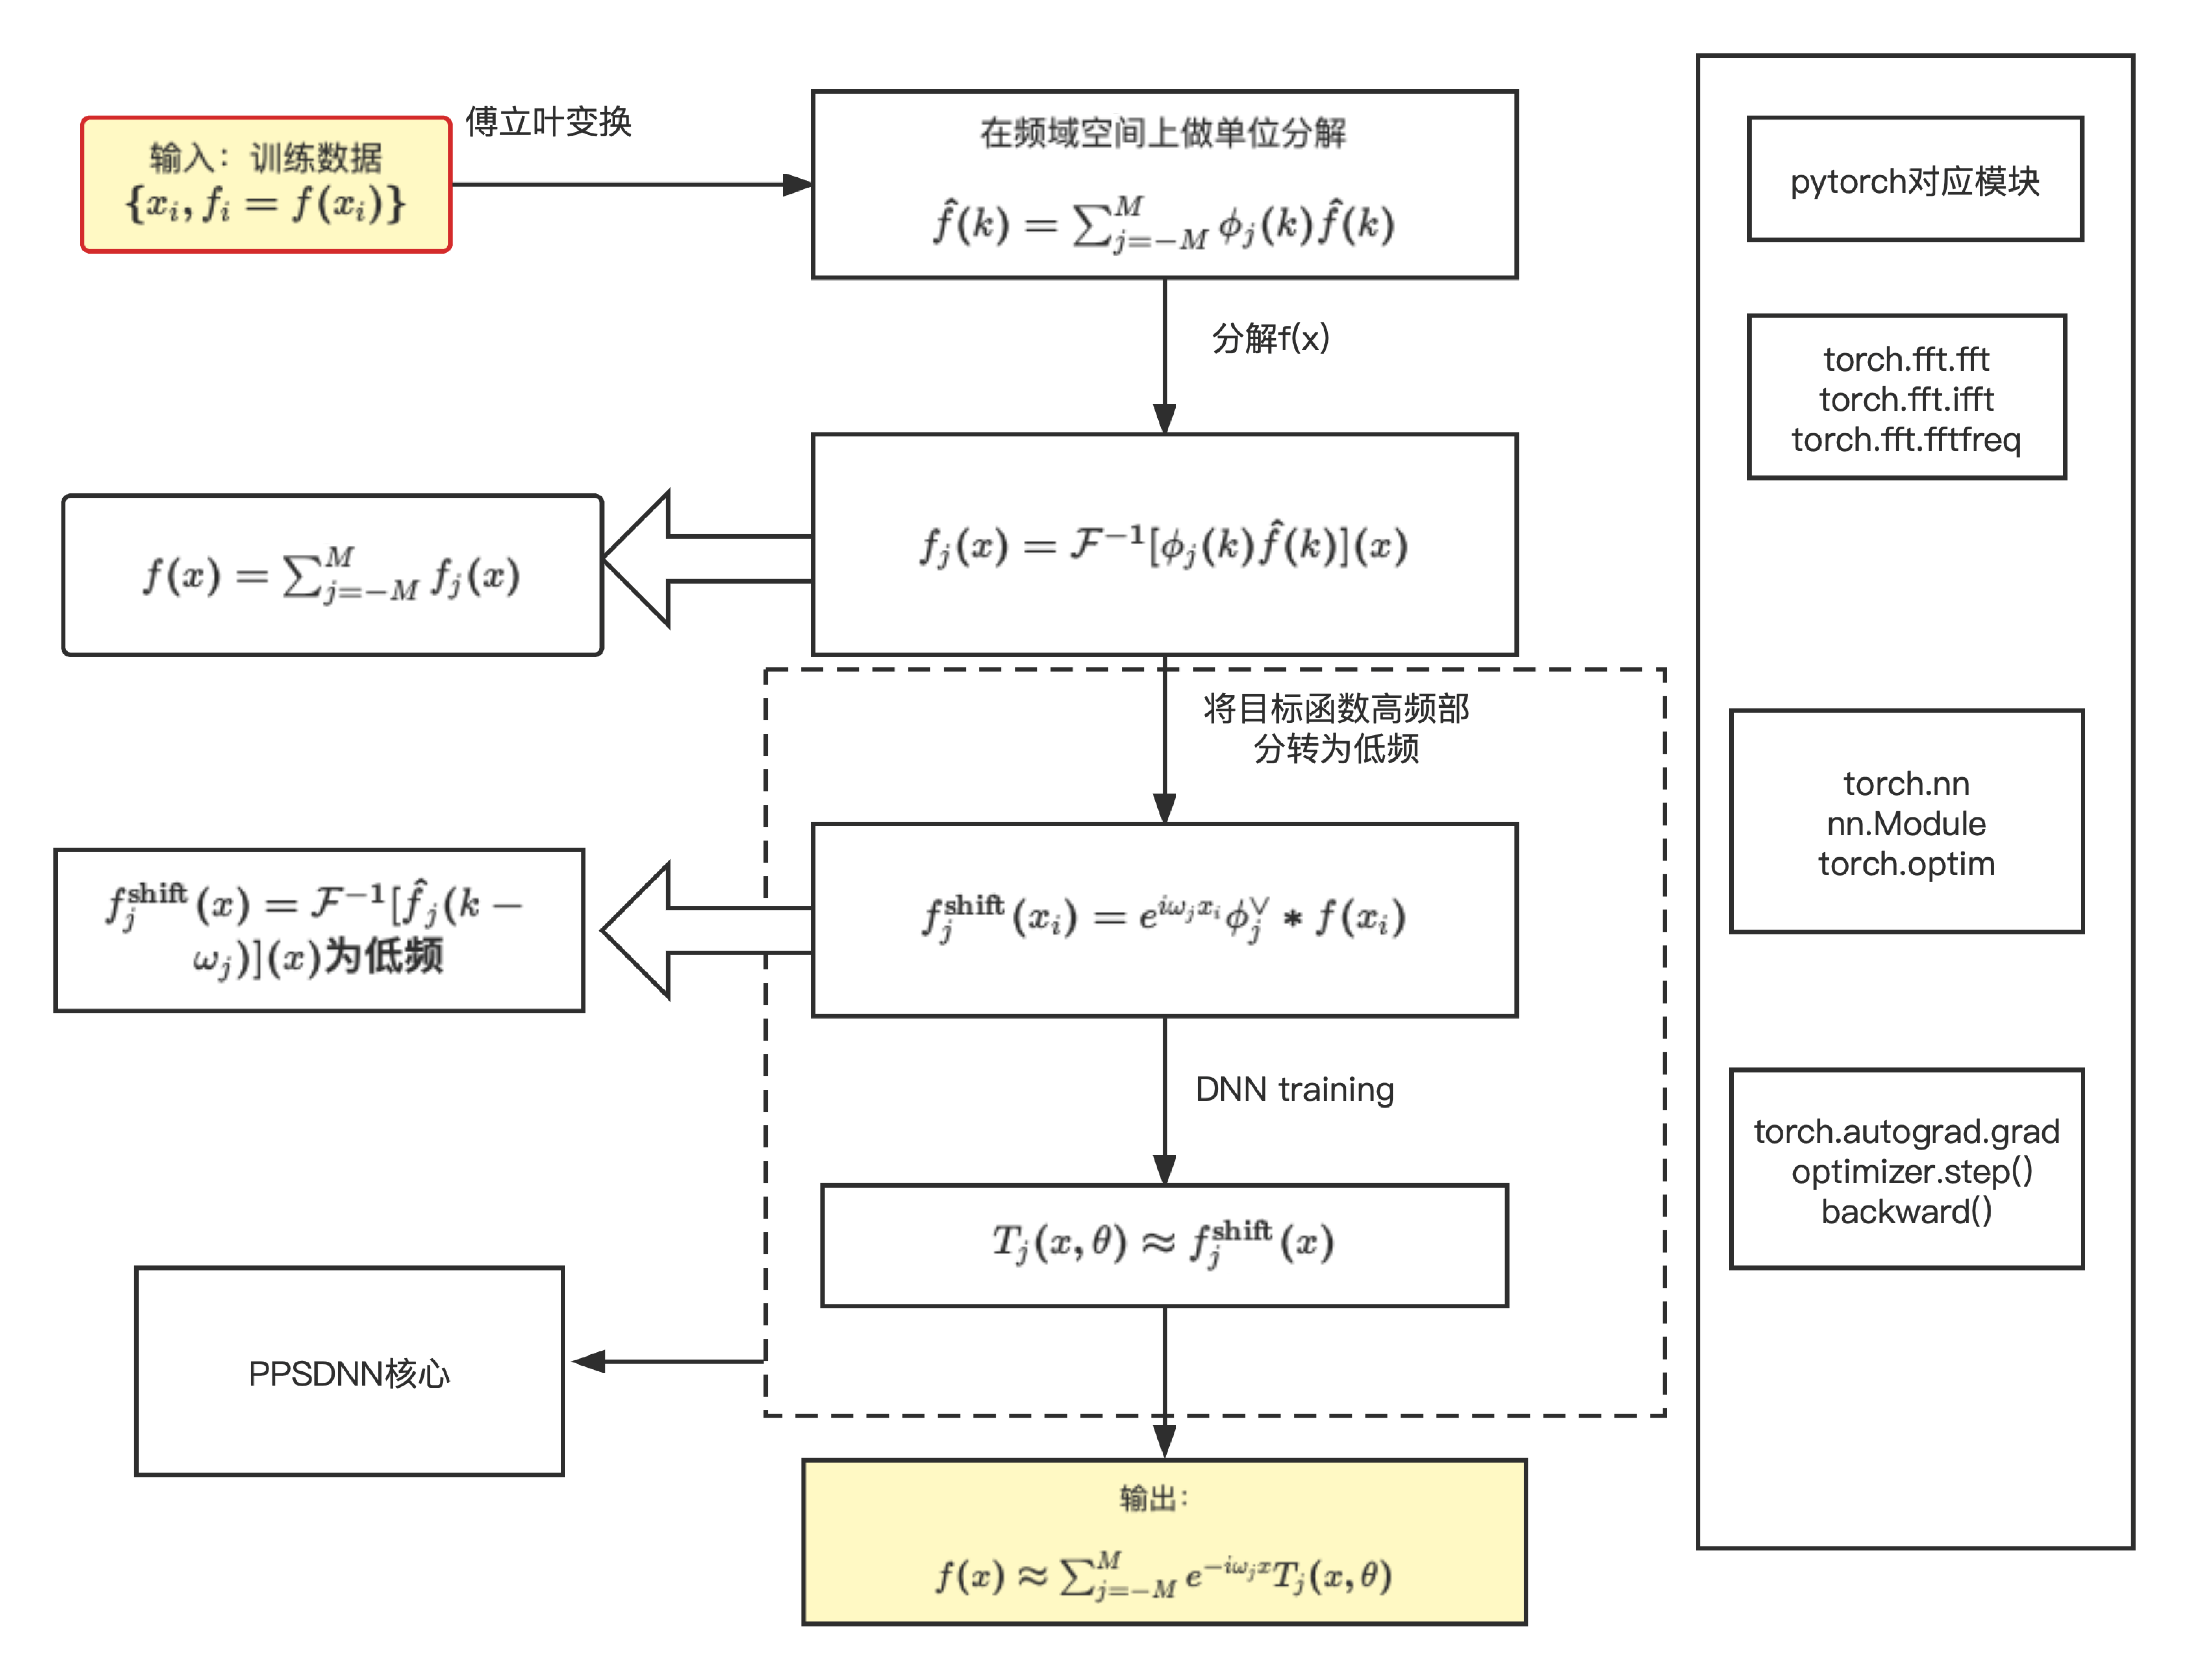
\includegraphics[width=0.95\linewidth]{figures/ppsdnnchart.pdf}
    \caption{PPSDNN算法流程图}
    \label{ppsdnnchart}
\end{figure}




%----------------------------------------------------------------------------------------------------------------
\chapter[初步结果]{初步结果}
\label{chap3}
\section{toy model测试结果}
下面通过两个数值例子介绍PPSDNN的算法实现以及一些更多的算法细节。第一个数值的例子是训练一个有确定函数形式生成的数据,且我们可以根据它的函数形式大致确定其频域空间的范围,在第一个例子中将引入和PPSDNN等价的另一种实现phase shift的方法。
第二个数值例子是训练一个不光滑的函数生成的数据,它的特点是根据函数形式无法大致确定其频域空间的范围,因此在第二个例子中引入频率扫荡方法(frequency sweep)。此外,PPSDNN还可以用来拟合多维的振荡数据,解高频的波动方程,亥姆霍兹方程等,但这些应用不在本文的范围之内。

首先介绍第一个数值例子。在第一个例子中,我们选取目标函数f(x)的定义域为$[-\pi,\pi]$,函数形式为
\begin{equation}\label{eq:target1}
    f(x) = \begin{cases}
             10(\sin x + \sin 3x), & \mbox{如果 } x\in [-\pi,0] \\
             10(\sin 23x + \sin 137x + \sin 203x), & \mbox{如果 }x\in [0,\pi].
           \end{cases}
  \end{equation}
在定义域上画出函数图形,如图\ref{toy}所示:
\begin{figure}[htbp]
  \centering
  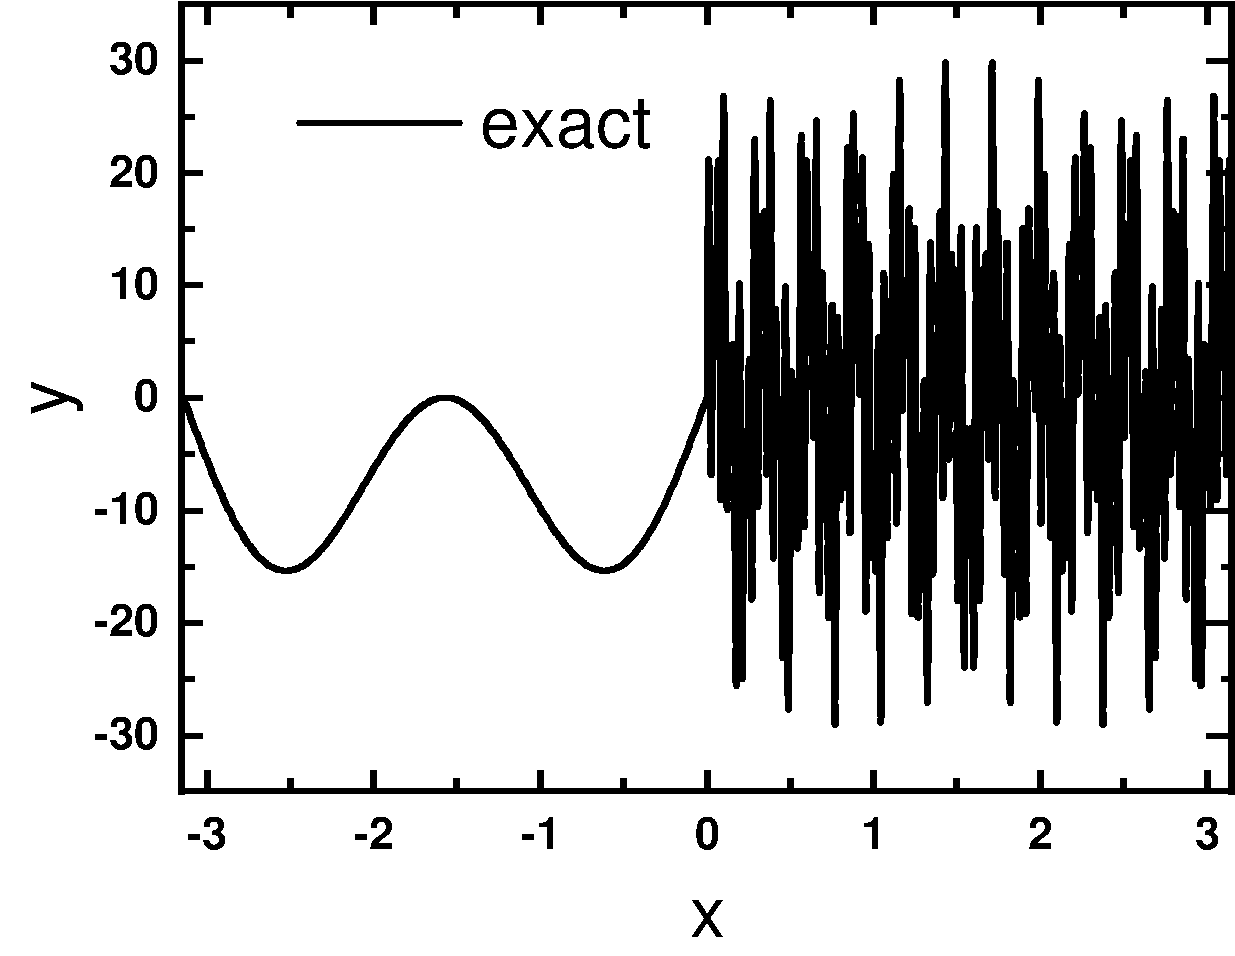
\includegraphics[width=0.76\linewidth]{figures/toymodel/exact.pdf}
  \caption{toy model目标函数\ref{eq:target1}式的图形}
  \label{toy}
\end{figure}

  因为该函数的频率空间可以从它的函数形式或通过傅里叶变换得到,因此我们取$\Delta k=5$,用以下的特征函数对目标函数进行单位分解。
  \begin{equation}\label{}
    \begin{aligned}
      &\phi_1(k) = \chi_{[-205,-200]}(k)  & \phi_2(k) = \chi_{[-140,-135]}(k)\\
      & \phi_3(k) = \chi_{[-25,-20]}(k)  & \phi_4(k) = \chi_{[-5,0]}(k)\\
      &\phi_5(k) = \chi_{[0,5]}(k)   & \phi_6(k) = \chi_{[20,25]}(k)\\
      & \phi_7(k) = \chi_{[135,140]}(k)  & \phi_8(k) = \chi_{[200,205]}(k)
      \end{aligned}
  \end{equation}
  则$f_j(x) = \mathcal{F}^{-1}[\widehat{f}\phi_j](x)$。训练DNN的参数为:
  \begin{itemize}
    \item DNN结构:1-40-40-40-40-1
    \item 训练集:函数定义域上均匀分布的10,000个数据点
    \item 测试集:函数定义域上均匀分布的1000个数据点
    \item epochs:1000
    \item 优化器:Adam
    \item 学习率:0.002
    \item batchsize:2000
  \end{itemize}

  训练结果如图\ref{sin},训练细节如图\ref{toy1},\ref{toy2},\ref{toy3}:
\begin{figure}[htbp!]
  \centering
  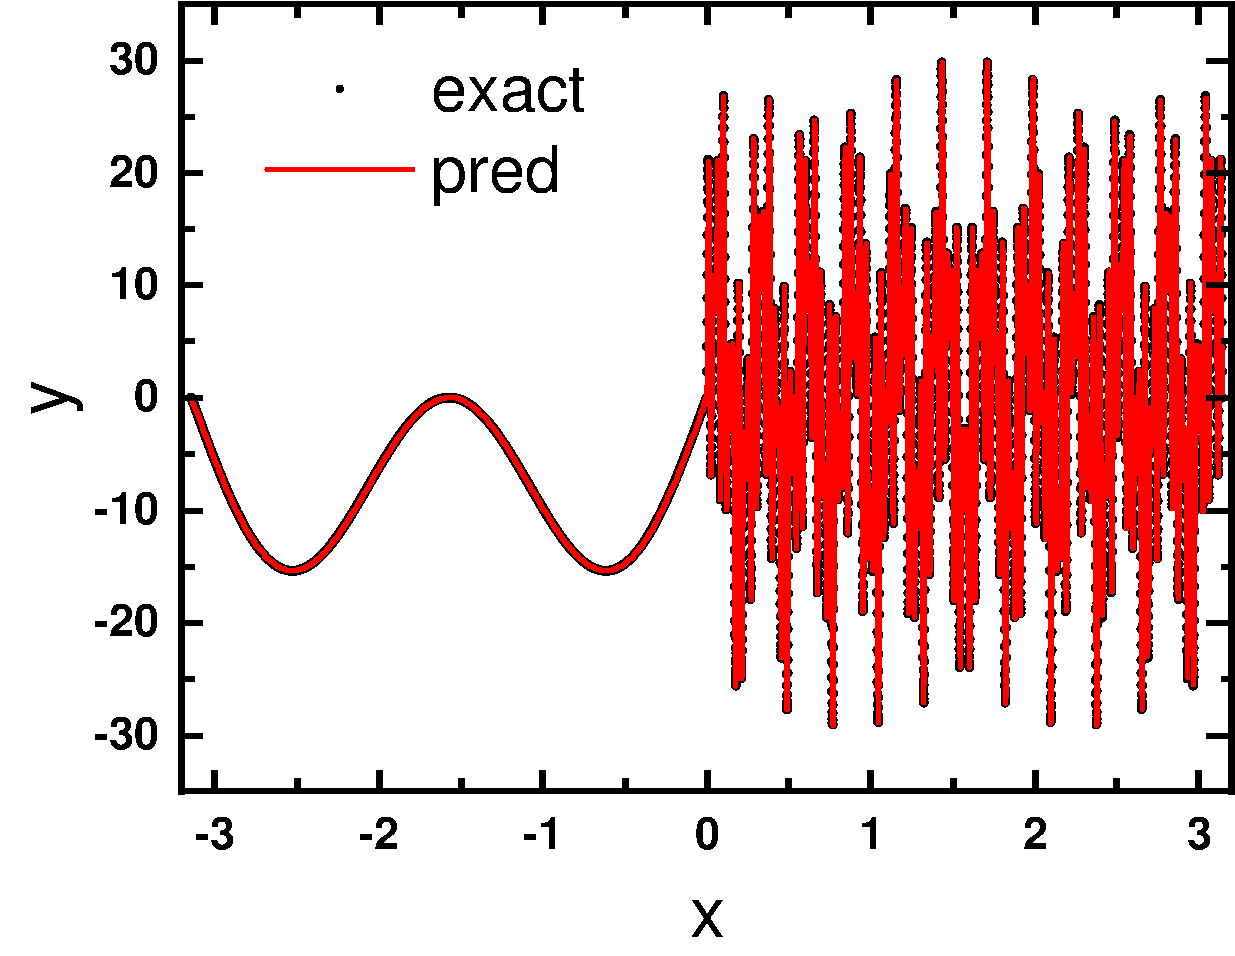
\includegraphics[width=0.77\linewidth]{figures/toymodel/train.pdf}
  \caption{使用PPSDNN训练目标函数\ref{eq:target1}式}
  \label{sin}
\end{figure}
\begin{figure}[htbp]
  \centering
  \includegraphics[width=0.76\linewidth]{figures/toymodel/train1.pdf}
  \caption{toy model在区间$[0,1]$上的训练细节}
  \label{toy1}
\end{figure}
\begin{figure}[htbp]
  \centering
  \includegraphics[width=0.76\linewidth]{figures/toymodel/train2.pdf}
  \caption{toy model在区间$[1,2]$上的训练细节}
  \label{toy2}
\end{figure}
\begin{figure}[htbp]
  \centering
  \includegraphics[width=0.76\linewidth]{figures/toymodel/train3.pdf}
  \caption{toy model在区间$[2,3.14]$上的训练细节}
  \label{toy3}
\end{figure}
  


  在PPSDNN中,由于频率选择核要与训练数据做卷积运算,因此,在高维的卷积运算中,它的空间复杂度为$O (N\times N)$,说明平行相移的方法存在维数灾难,为了避免这个问题,人们提出了Coupled Weighted phase shift DNN\cite{cai2020phase}(CPSDNN):
  \begin{equation} \label{eq:CPDNNcomplex}%
    T(x)=\sum_{m=1}^{M}e^{i\omega_{m}x}T_{m}(x),
    \end{equation}
    其中$\{\omega_{m}\}_{m=1}^M$是和目标函数有关的频率空间。将指数项写成实数的形式为
    \begin{equation}\label{eq:CPDNNreal}%
      T(x)=\sum_{m=1}^{M}A_{m}\cos(\omega_{m}x)+B_{m}\sin(\omega_{m}x)
      \end{equation}
    于是,我们可以定义并最小化损失函数:
    \begin{equation}
      \begin{aligned}
      L(\theta) &= \int_{-\infty}^{+\infty}|f(x)-T(x)|^2d x,\label{eq:2}%
      \end{aligned}
      \end{equation}
      在离散情况下可以写成:
      \begin{equation}
        L_N(\theta) = \sum_{i=1}^{N}\left\vert
        f(x_{i})-T(x_{i})\right\vert ^{2}
        =\sum_{i=1}^{N}\left\vert f(x_{i})-\sum_{m=1}^{M}e^{i\omega_{m}x_{i}}T_{m}(x_{i})\right\vert ^{2}. \label{eq:Ln2}%
        \end{equation}
在实际应用中,我们往往引入正则项,于是损失函数可以改写为
\begin{equation}
  L_N^R(\theta) = \sum_{i=1}^{N}|f(x_i) - T(x_i)|^2 + \beta \sum_{m,l} \norm{\vec{W}^{m, l}}_F^2.
  \end{equation}
  其中,$\beta$是正则化参数,$\vec{W}^{m, l}$是$T_m$的权重矩阵。可以证明,PPSDNN方法和CPSDNN方法训练效果是等价的,而CPSDNN来源于PPSDNN算法的启发。

%   当使用CPSDNN训练第一个例子是,我们选取$\{\omega_{m}\}=\{0,5,25,135,200\}$,其他参数和PPSDNN相同。
%   下面图\ref{1D-10000}是普通DNN方法和CPSDNN方法对第一个数值例子的训练结果比较。
% \begin{figure}[htbp!]
%   \centering
%   \includegraphics[width=0.84\linewidth]{figures/PPSDNN/1D-10000.pdf}
%   \caption{普通DNN和CPSDNN对高频目标函数训练的比较}
%   \label{1D-10000}
% \end{figure}

下面介绍第二个数值例子。在实际工作中,我们学习的核数据一般都是离散的,不像第一个例子生成的函数是连续且光滑的。这时候我们就要用到频率扫荡(frequency sweep)方法。前面取的$\omega _m$都是几个离散的值,在frequency sweep中,我们可以取形如$\omega _m=-1600:10:1600$这样连续的值。我们将\ref{eq:target1}的函数稍作修改,将x小于零的部分改成阶跃函数,使它的频率空间不再那么确定,接着使用frequency sweep进行训练。

训练效果如图\ref{sweep}
\begin{figure}[htbp!]
  \centering
  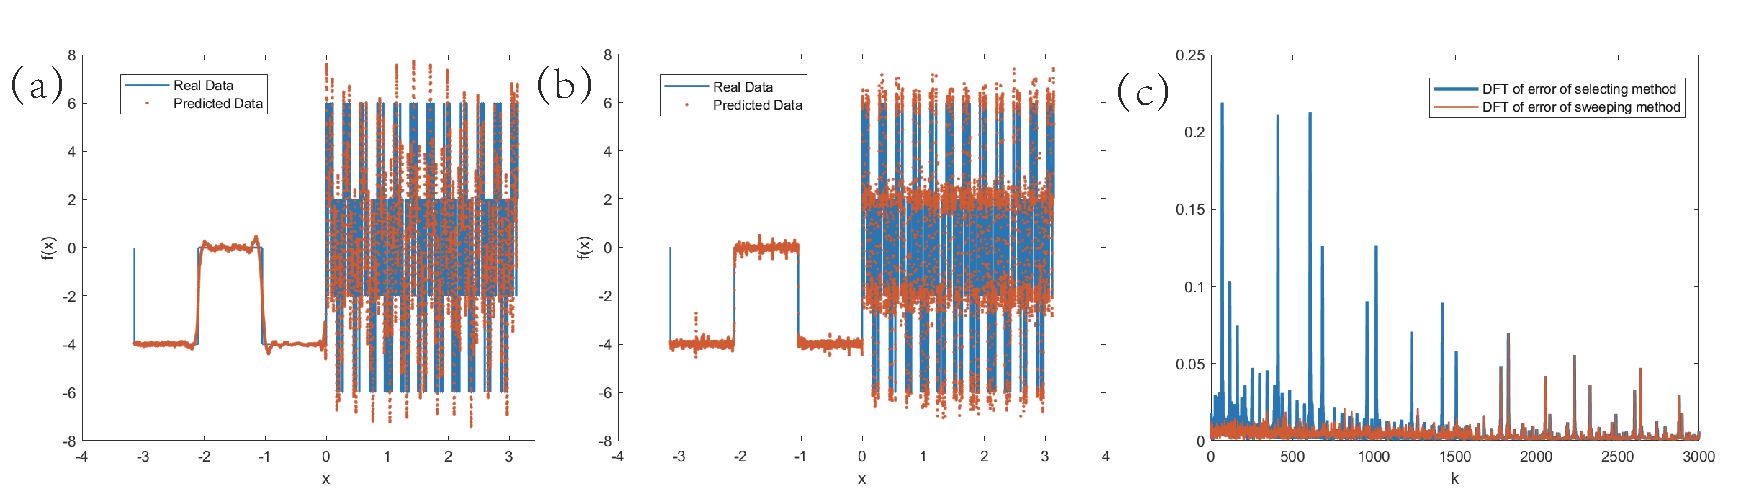
\includegraphics[width=0.84\linewidth]{figures/PPSDNN/1D-square.pdf}
  \caption{使用frequency sweep训练高频函数}
  \label{sweep}
\end{figure}


\section{$^{235}\text{U}(n,f)$评价库数据测试结果}
根据核反应的复合核理论,当中子与靶核形成复合核时,复合核的激发能为
\begin{equation}\label{}
  E^{\ast } = \frac{m_A}{m_n+m_A}E_n+B_{nA}
\end{equation}
其中,$m_A$为靶核的质量,$m_n$为中子的质量,$E_n$为入射中子的相对动能,$B_{nA}$为中子与靶核的结合能。当形成的复合核能级等于$E^{\ast }$时,入射粒子被强烈吸收,形成共振峰。
% 在此工作中,我们以$^{235}\text{U}(n,f)$反应为例,使用PPSDNN方法,对其截面数据进行学习研究。此反应的实验数据和ENDF/B-VIII.0评价库的数据如图\ref{u235expendf}所示.

近几十年以来,$^{235}\text{U}$中子共振区的实验测量和理论研究一直是生机勃勃的,累计的实验截面数据估计在10万以上。由于测量技术,参数分析方法的不同,共振参数间存在着分歧。同时,一家测量分析的结果往往不能覆盖全部能区和给出全部共振参数。因此,综合多家实验数据进行分析评价是十分必要的\cite{何锦昌1990中子共振参数的联合拟合分析}。而目前最核心的技术难题就是难以拟合好高频振荡的数据。在$\text{n}+^{235}\text{U}$反应中,存在多种截面数据,包括裂变截面,俘获截面,全截面等。本工作研究的是裂变截面。


ENDF/B-VIII.0是美国核反应数据库ENDF的最新版本,于2018年2月2日发布\cite{Brown2018}。它完全采用了新的中子数据标准,改进了热中子散射数据,并使用了国际评价库组织(CIELO)试点项目的新评价数据,涵盖了氢、氧、铁、铀和钚等元素的中子反应\cite{Sobes2021}。由于评价库中的核数据与实验核数据相比,其截面数据的连续性与光滑性更好,因此更适合使用神经网络方法进行学习。
下面将分别使用普通DNN方法和PPSDNN方法学习这些实验数据以及评价库中的数据。



在此部分,首先介绍普通DNN方法在研究$^{235}\text{U}(n,f)$反应中的应用。根据第二章的分析,由于f- principle,DNN方法更偏向于先学习低频数据,再学习高频数据,因此,在中子共振区域,在有限运算资源的情况下,DNN方法的学习效果并不会很好。

由于实验数据每家测量的分歧较大,因此为了快速从实践上验证PPSDNN在中子共振中应用的可行性,本文采用ENDF/B-VIII.0的数据作为学习数据集。
下面是使用PPSDNN方法对$^{235}\text{U}(n,f)$反应的评价库数据进行学习的结果。
% 下面是使用ENDF/B-VIII.0库的学习结果。如图
\begin{figure}[htbp!]
  \centering
  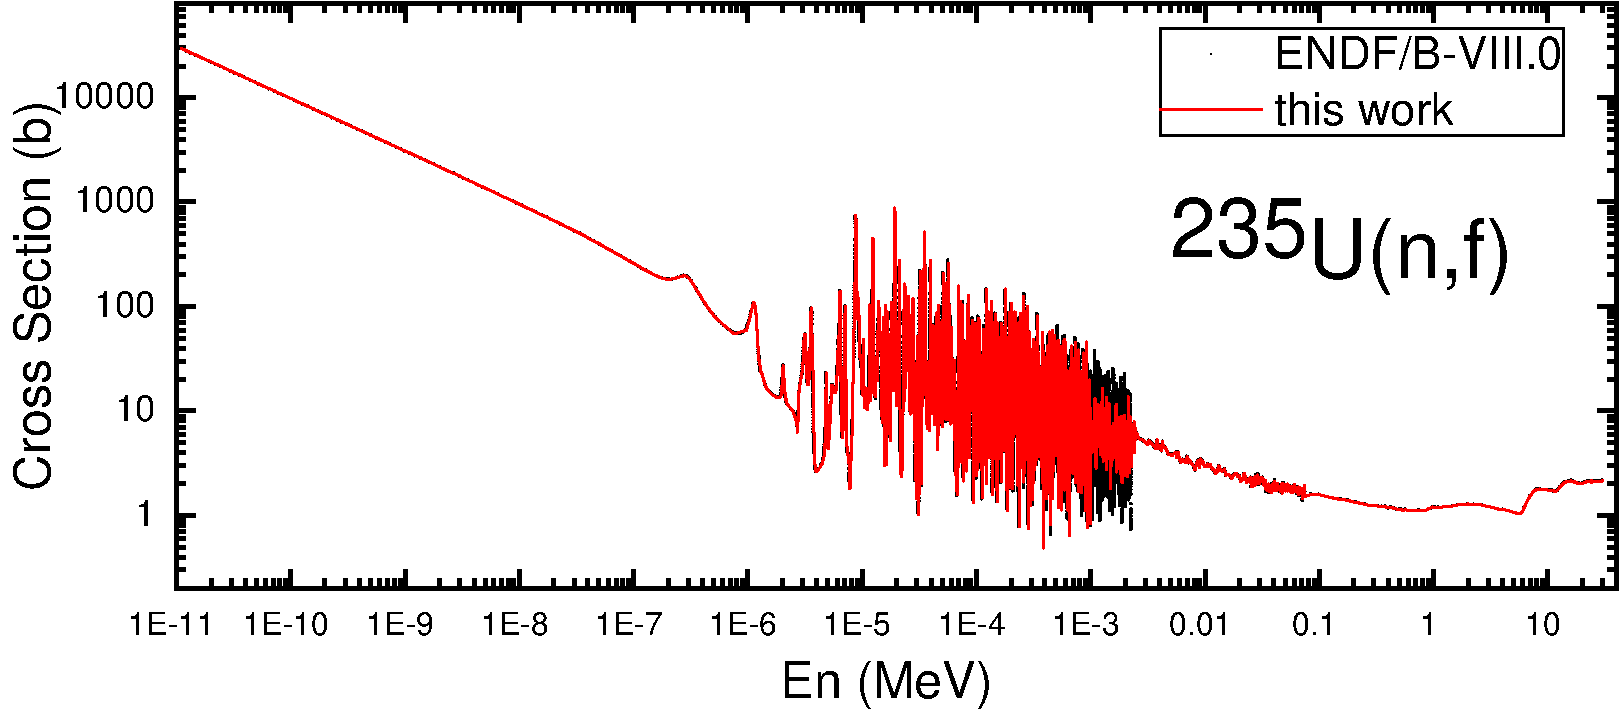
\includegraphics[width=0.94\linewidth]{figures/endftrain/endftrain.pdf}
  \caption{PPSDNN方法对ENDF/B-VIII.0数据库中$^{235}\text{U}(n,f)$反应截面的学习}
  \label{endftrain}
\end{figure}
\begin{figure}[htbp!]
  \centering
  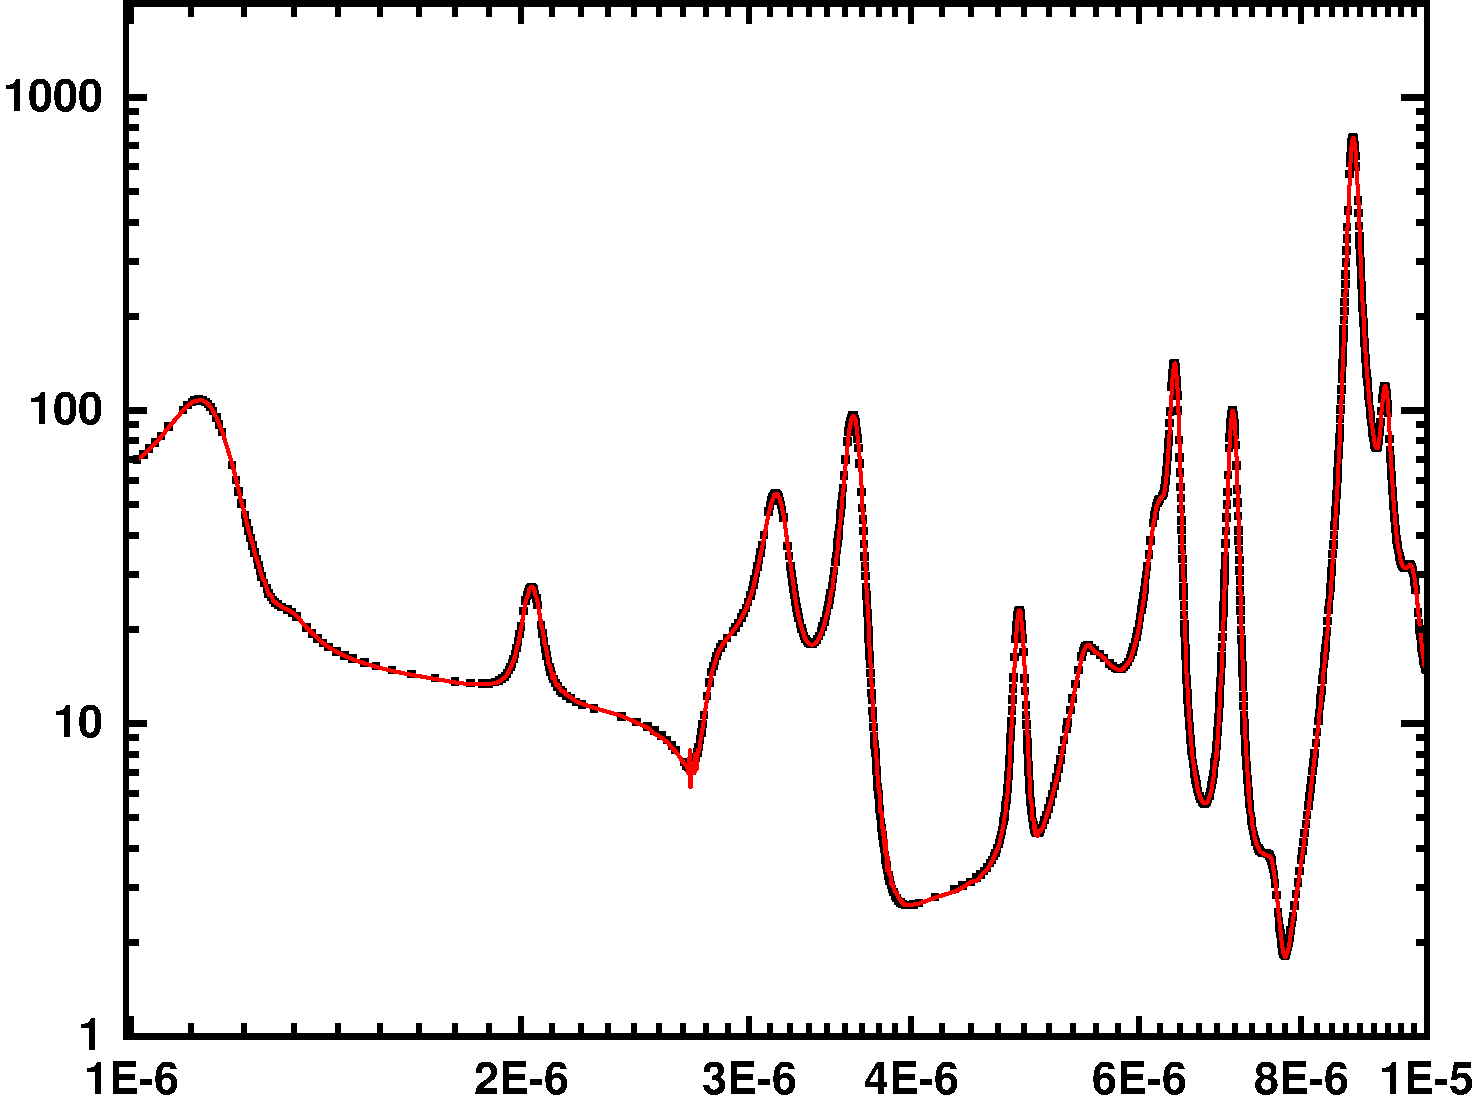
\includegraphics[width=0.84\linewidth]{figures/endftrain/G6.pdf}
  \caption{PPSDNN方法在能量区间为$[10^{-6},10^{-5}]$MeV的学习细节}
  \label{endf6}
\end{figure}
\begin{figure}[htbp!]
  \centering
  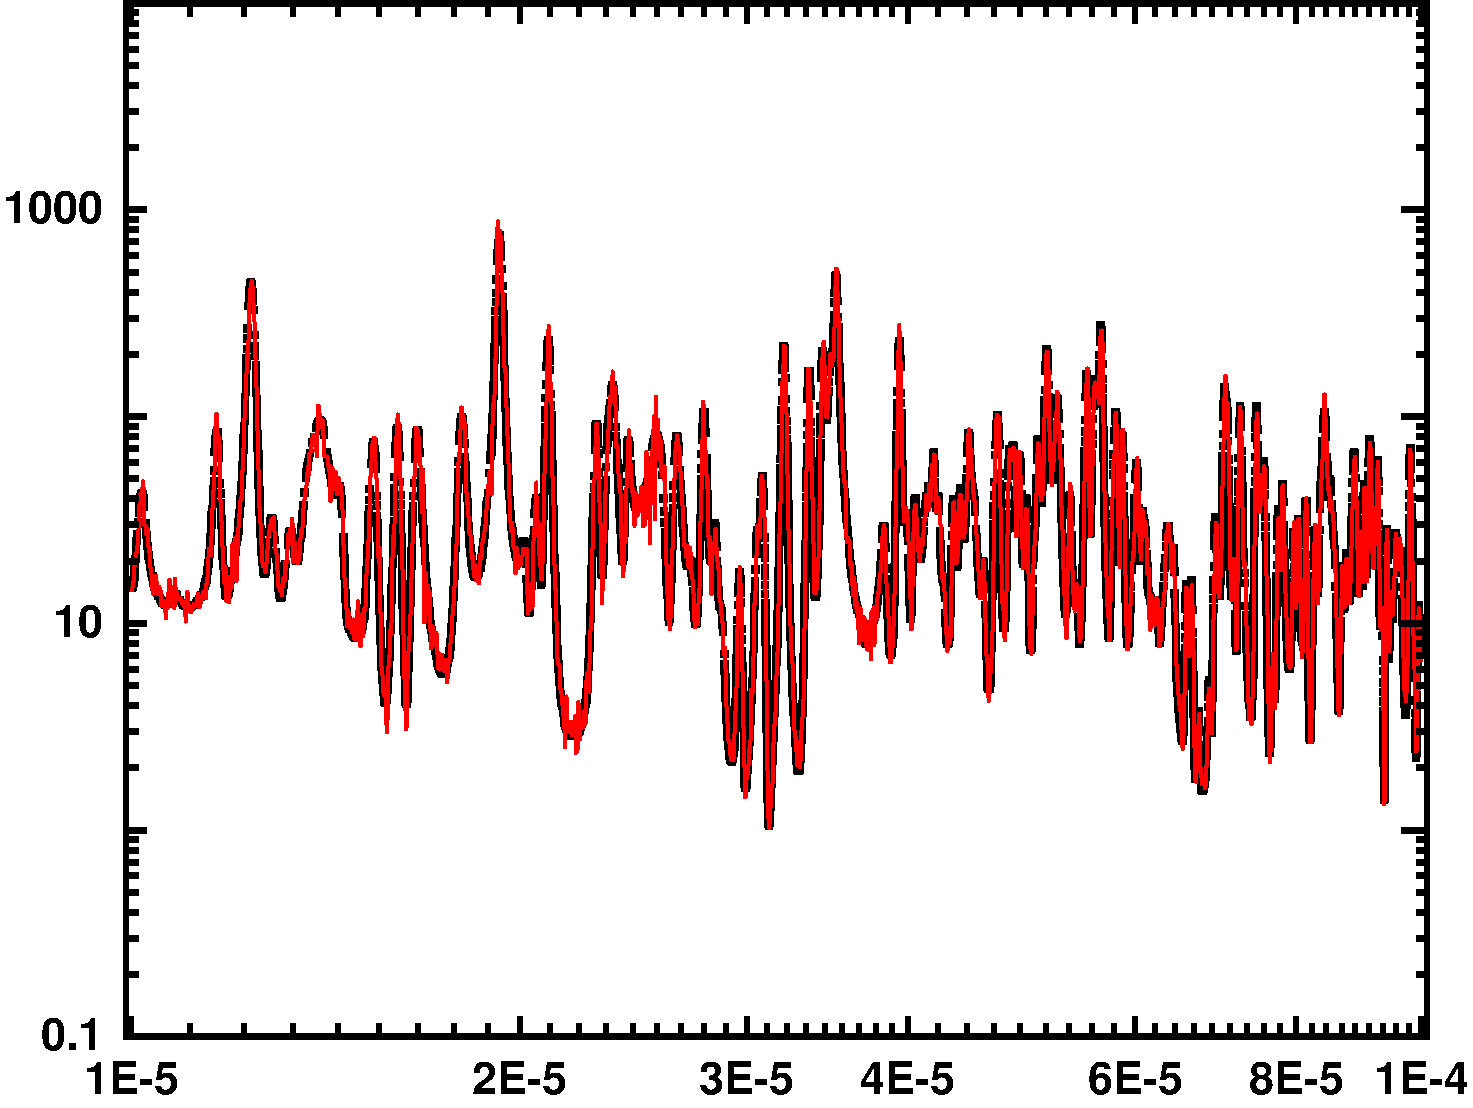
\includegraphics[width=0.84\linewidth]{figures/endftrain/G5.pdf}
  \caption{PPSDNN方法在能量区间为$[10^{-5},10^{-4}]$MeV的学习细节}
  \label{endf5}
\end{figure}
\begin{figure}[htbp!]
  \centering
  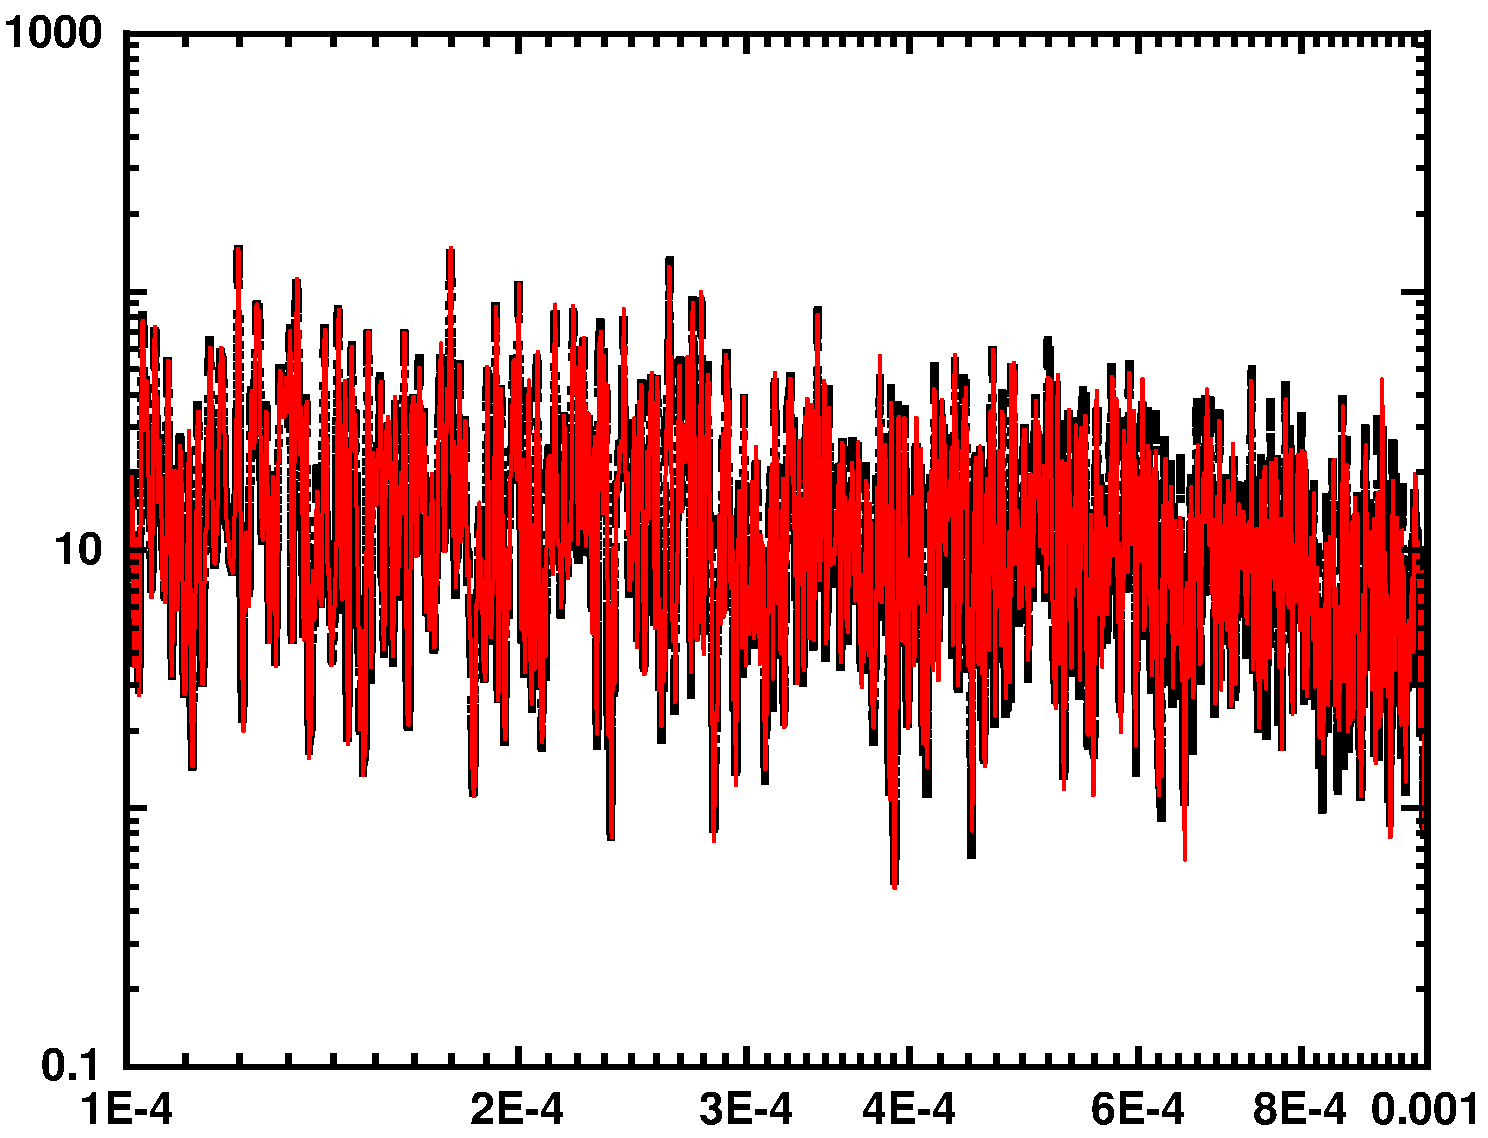
\includegraphics[width=0.84\linewidth]{figures/endftrain/G4.pdf}
  \caption{PPSDNN方法在能量区间为$[10^{-4},10^{-3}]$MeV的学习细节}
  \label{endf4}
\end{figure}
\begin{figure}[htbp!]
  \centering
  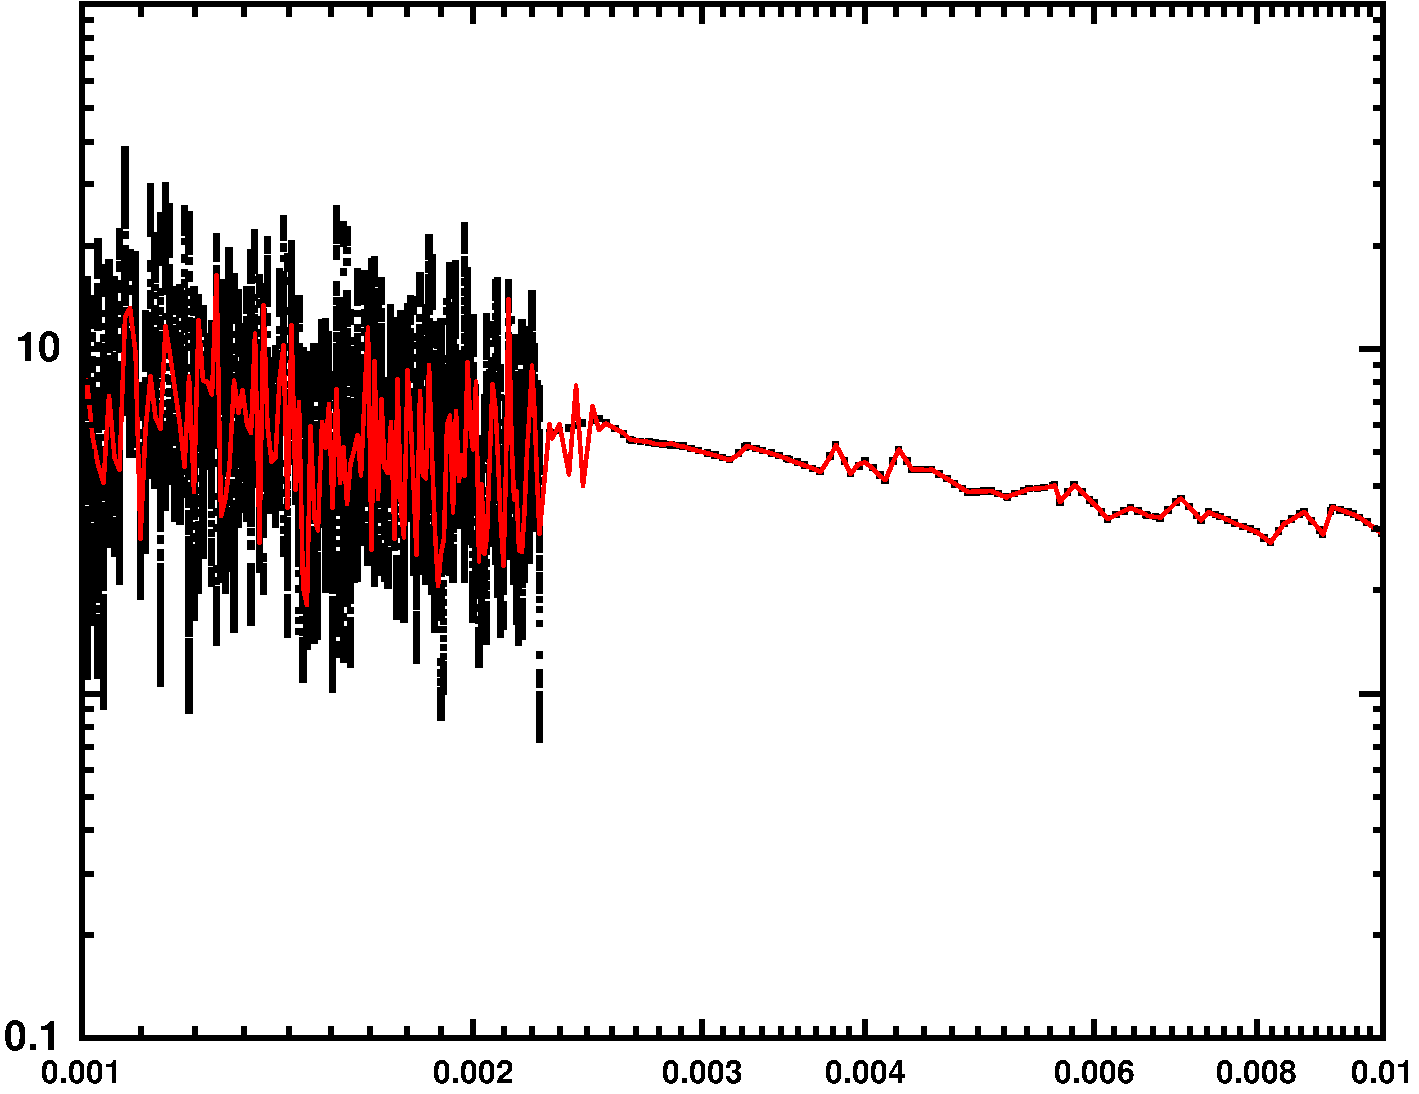
\includegraphics[width=0.84\linewidth]{figures/endftrain/G3.pdf}
  \caption{PPSDNN方法在能量区间为$[10^{-3},10^{-2}]$MeV的学习细节}
  \label{endf3}
\end{figure}
\begin{figure}[htbp!]
  \centering
  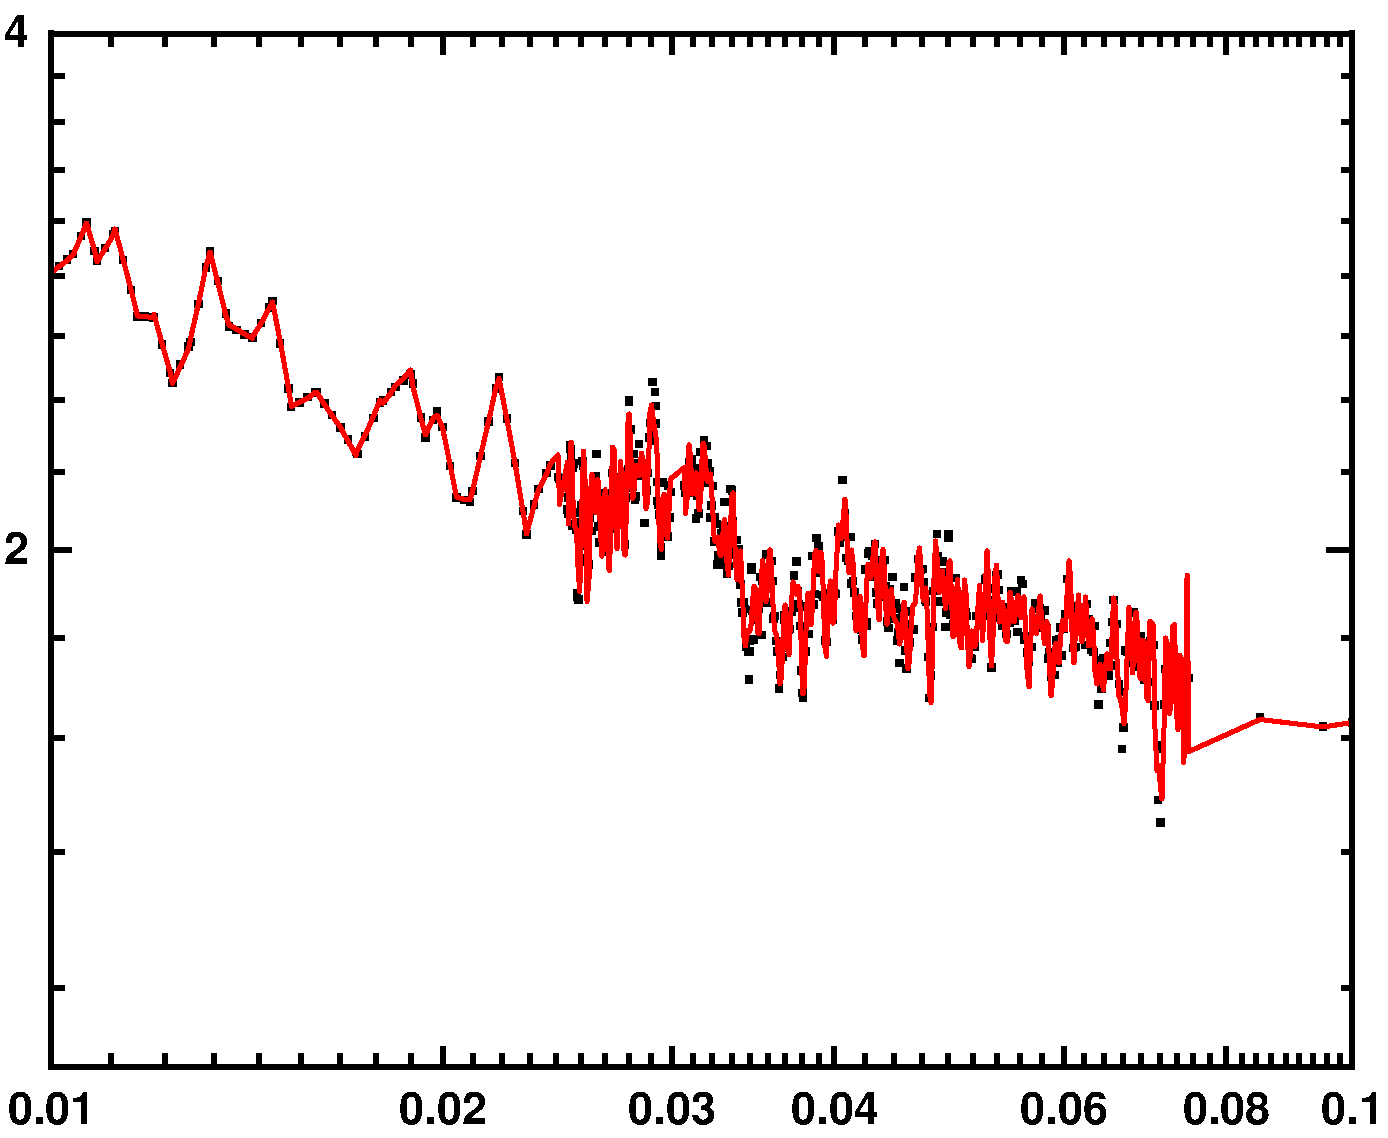
\includegraphics[width=0.84\linewidth]{figures/endftrain/G2.pdf}
  \caption{PPSDNN方法在能量区间为$[10^{-2},10^{-1}]$MeV的学习细节}
  \label{endf2}
\end{figure}
\begin{figure}[htbp]
  \centering
  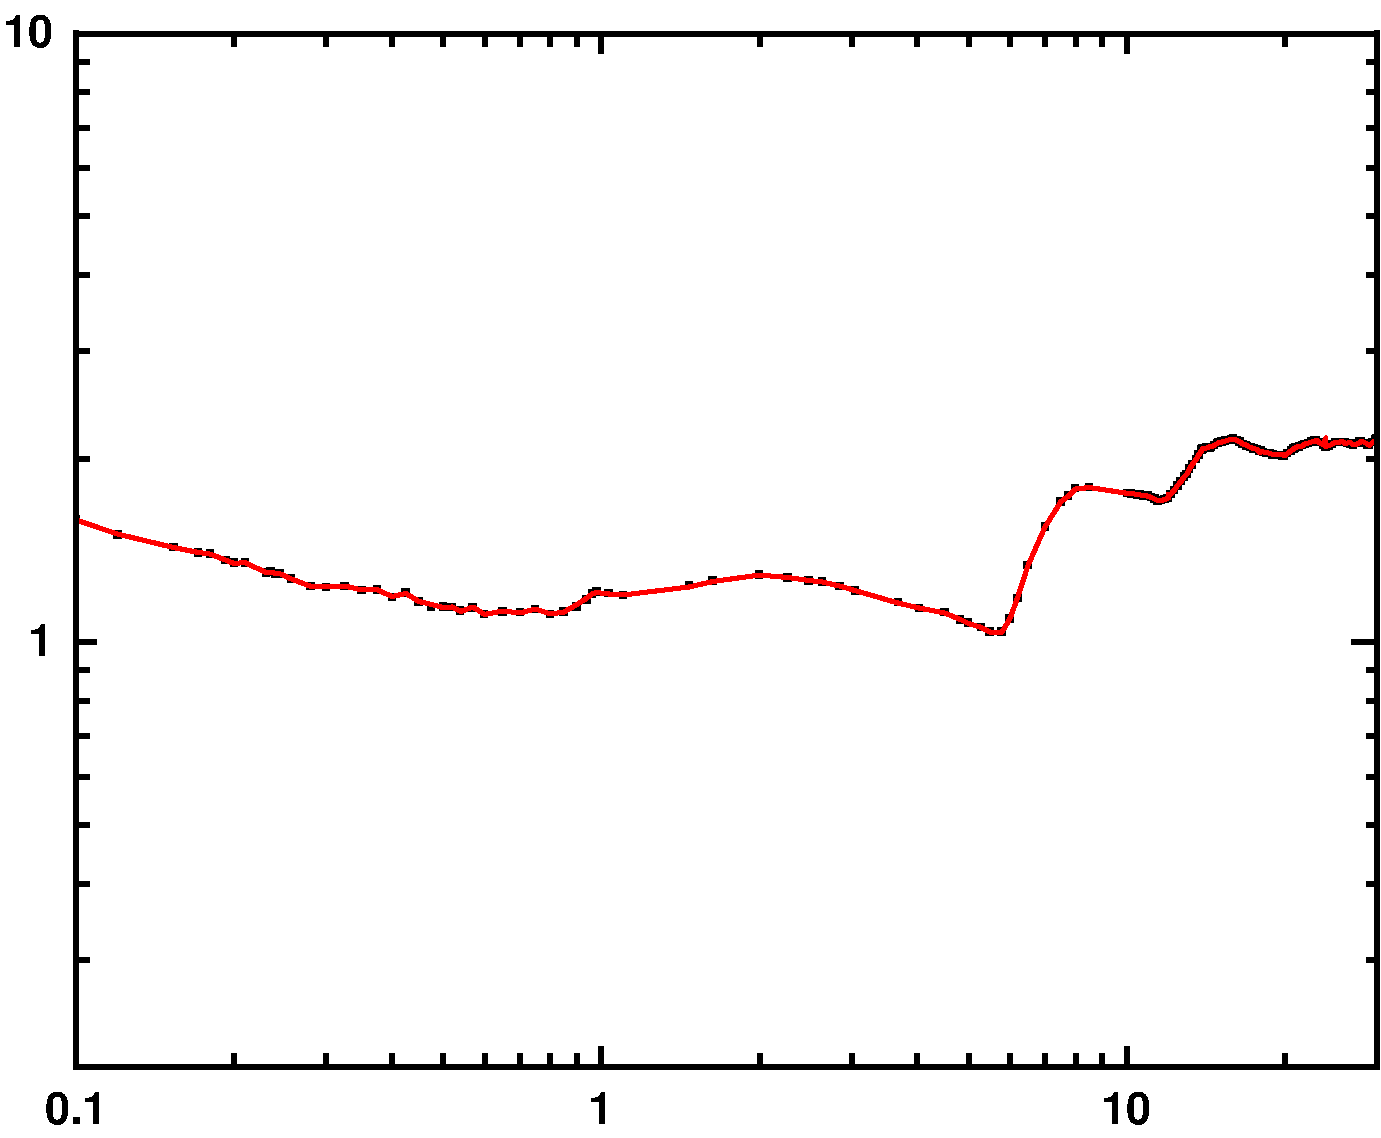
\includegraphics[width=0.84\linewidth]{figures/endftrain/G1.pdf}
  \caption{PPSDNN方法在能量区间为$[0.1,30]]$MeV的学习细节}
  \label{endf1}
\end{figure}
从图中可以看出,PPSDNN可以较好地学习到入射能为$10^{-6}\thicksim 0.001$MeV共振区的评价库数据。当入射能超过0.001MeV时,可以用来学习的数据量大大减少,且接近不可分辨共振区,因此会在一小段能区无法重现评价库数据。当能量大于0.003MeV时,PPSDNN可以学习到不可分辨共振区的数据。


由于评价库的核数据和实验数据相比更具有光滑性,而我们的目的是根据实验数据给出一套自己的核数据评价方法。因此后续将尝试使用PPSDNN方法直接学习$^{235}\text{U}(n,f)$反应截面的实验数据。
% 下面是学习结果

% 等结果跑出来ing






 %--------------------------------------------------------------
\chapter{总结与展望}\label{chap4}
% 这是我毕业论文的总结和展望部分:

本文详细推导并复现了PPSDNN算法,实现了PPSDNN算法对toy model的学习,在toy model中,目标函数是连续可导的,其傅立叶变换也是解析的,根据其傅立叶变换得到的采样频率,通过平行相移,就可以很好的学习toy model。在实际应用中,训练数据是离散的,比如$^{235}\text{U}(n,f)$反应的评价数据,通过frequency sweep,也可以做到较好的学习这类离散数据。这表明该算法确实具有较高的预测精度和效率和较好高频数据学习能力。
这为今后从事中子共振截面的评价工作奠定了坚实的基础。

机器学习用于中子共振研究还有以下潜在应用:
\begin{enumerate}
    \item 加速计算\cite{verbraeken2020survey}。中子共振计算中需要进行大量的矩阵运算和复杂的数值计算,通常非常耗时。使用机器学习算法,可以通过对之前计算过的数据进行训练,从而加速计算过程并保持相同的计算精度。
    \item 提高计算精度。中子共振计算中存在着一些难以处理的误差和不确定性。使用机器学习算法可以通过对大量数据进行训练,从而减小误差和降低不确定性,提高计算精度。
    \item 数据分析。中子共振实验通常产生大量数据,如能谱和截面等。使用机器学习算法,可以对这些数据进行分析和分类,更好地理解中子共振现象和物理机制。
    \item 拟合物理模型参数。中子共振研究中需要对物理模型进行拟合,以更好地描述中子共振现象和物理机制。使用机器学习算法,可以对大量的实验数据进行训练,以获得更好的拟合效果和更准确的模型参数。随着中子共振核反应数据量的增加,机器学习方法也逐渐体现出其独有的优势。
\end{enumerate}

在今后的工作中,将继续发挥机器学习的优势,并将PPSDNN方法用于学习以$^{235}\text{U}(n,f)$反应为代表的中子共振实验数据中。并使用学习和预言得到的激发曲线给出核反应的共振参数。

目前得到共振参数的主流方法是使用R矩阵拟合实验数据。
尽管R矩阵方法已经被广泛应用,但仍然存在一些困难和限制。例如,该方法只能唯象地给出道半径R,无法清晰地解释反应机制,而且R矩阵程序的编写也较为困难。为此,在今后的科研中计划将PPSDNN方法和R矩阵相结合,以改进共振参数的计算方法。这一方法将利用PPSDNN算法的高预测精度和高效率,以及R矩阵的核反应共振的原理,提高共振参数的准确性和高效性。
%\setcounter{secnumdepth}{0}%%编号深度,0为只对chaptter编号,section不编号
%\setcounter{tocdepth}{0}%%目录深度,但不知为何不起作用

\appendix

\renewcommand{\theequation}{\Alph{chapter}-\arabic{equation}}
\renewcommand{\thesubsubsection}{\arabic{subsubsection}.}
\setcounter{secnumdepth}{3}
%\addtocontents{toc}{\protect\setcounter{tocdepth}{0}}%%%没有tocvsec2宏包时可用这个
%\renewcommand\thesubsubsection{\arabic{subsubsection}}
% \settocdepth{chapter}
% \settocdepth{chapter}
\chapter{证明CPSDNN与PPDSNN的等价性}
\label{appendices a}
% \section{$C_{ij}$系数的计算过程}
% \subsection{$\pi\Xi\to\pi\Xi$}

由于交叉对称性,可以把末态的粒子变成初态上动量相反的反粒子

\clearpage
\phantomsection
\addcontentsline{toc}{chapter}{参考文献}
\bibliographystyle{gbt7714-numerical}
% \bibliography{standard}
% \bibliographystyle{whl}
\bibliography{b}
\backmatter%后记部分,页码格式不变,继续正常计数;其后的\chapter 不编号。
\titlecontents{chapter}[-4pt]{\addvspace{0pc}\heiti\sihao}{}{}{}
\clearpage
\phantomsection
\addcontentsline{toc}{chapter}{致谢}
\newpage
\thispagestyle{empty}
\fontsize{12pt}{13pt}\selectfont
\begin{center}\label{zhixie}
	{\xiaoerhao\textbf{致~~~~谢}}
\end{center}

\begin{flushleft}
\setlength{\parindent}{2em}
\hspace{1.6em}
% 虽然写论文的过程一直都是绝望阴暗的,但写到致谢部分已经变成希望明快的了。
我在此向所有在我硕士论文完成过程中提供支持和帮助的人们致以诚挚的感谢和敬意。

首先,我要向我的导师孙小军教授表达最真挚的感谢之情。导师不仅在研究过程中给予我专业而精准的指导和建议,更是以身作则,教会我如何做一个有追求、有担当的科研工作者。导师在我人生道路上的指引和支持,将成为我前行的力量和动力,使我更加坚定迈向未来的信心和决心。

其次,我要感谢罗秋莲等计算物理组的师兄师姐们,感谢他们在我研一时的帮助和支持。我还要感谢我的同门彭海圆师兄,梁艳师姐,张凯师兄,蓝秀丽师姐,邹方磊,唐诺程,崔嫣然,曹寒梅。另外,我还要感谢姚红师兄,万梦婷,杨赟,张国峰,陈立欣,陈叶若溪,李文琳,莫腾欢等核组的同学,我研究生大部分时间都是和他们一起度过的。以上这些人为我提供了最基础、最实用的技术支持,让我可以在学术中尽情发挥。他们严谨的治学态度、乐观向上的精神,都在潜移默化中影响和鼓励着我。

此外,我要感谢我的家人和朋友们,感谢他们在我完成学业的道路上给予我物质上的鼓励和支持。正是有了你们的陪伴和支持,我才有了追求知识和实现梦想的勇气和动力。谢谢你们的默默付出,是你们的陪伴,让我更坚定地走向自己的梦想之路。

另外,我要感谢一只特别的小生命——薛咪。她是我在研究生期间被收养的一只流浪猫。她的出现给了我无穷的欢乐和慰藉。
这张照片是薛咪在监督我写程序。
\begin{figure*}[htbp]
	\centering
	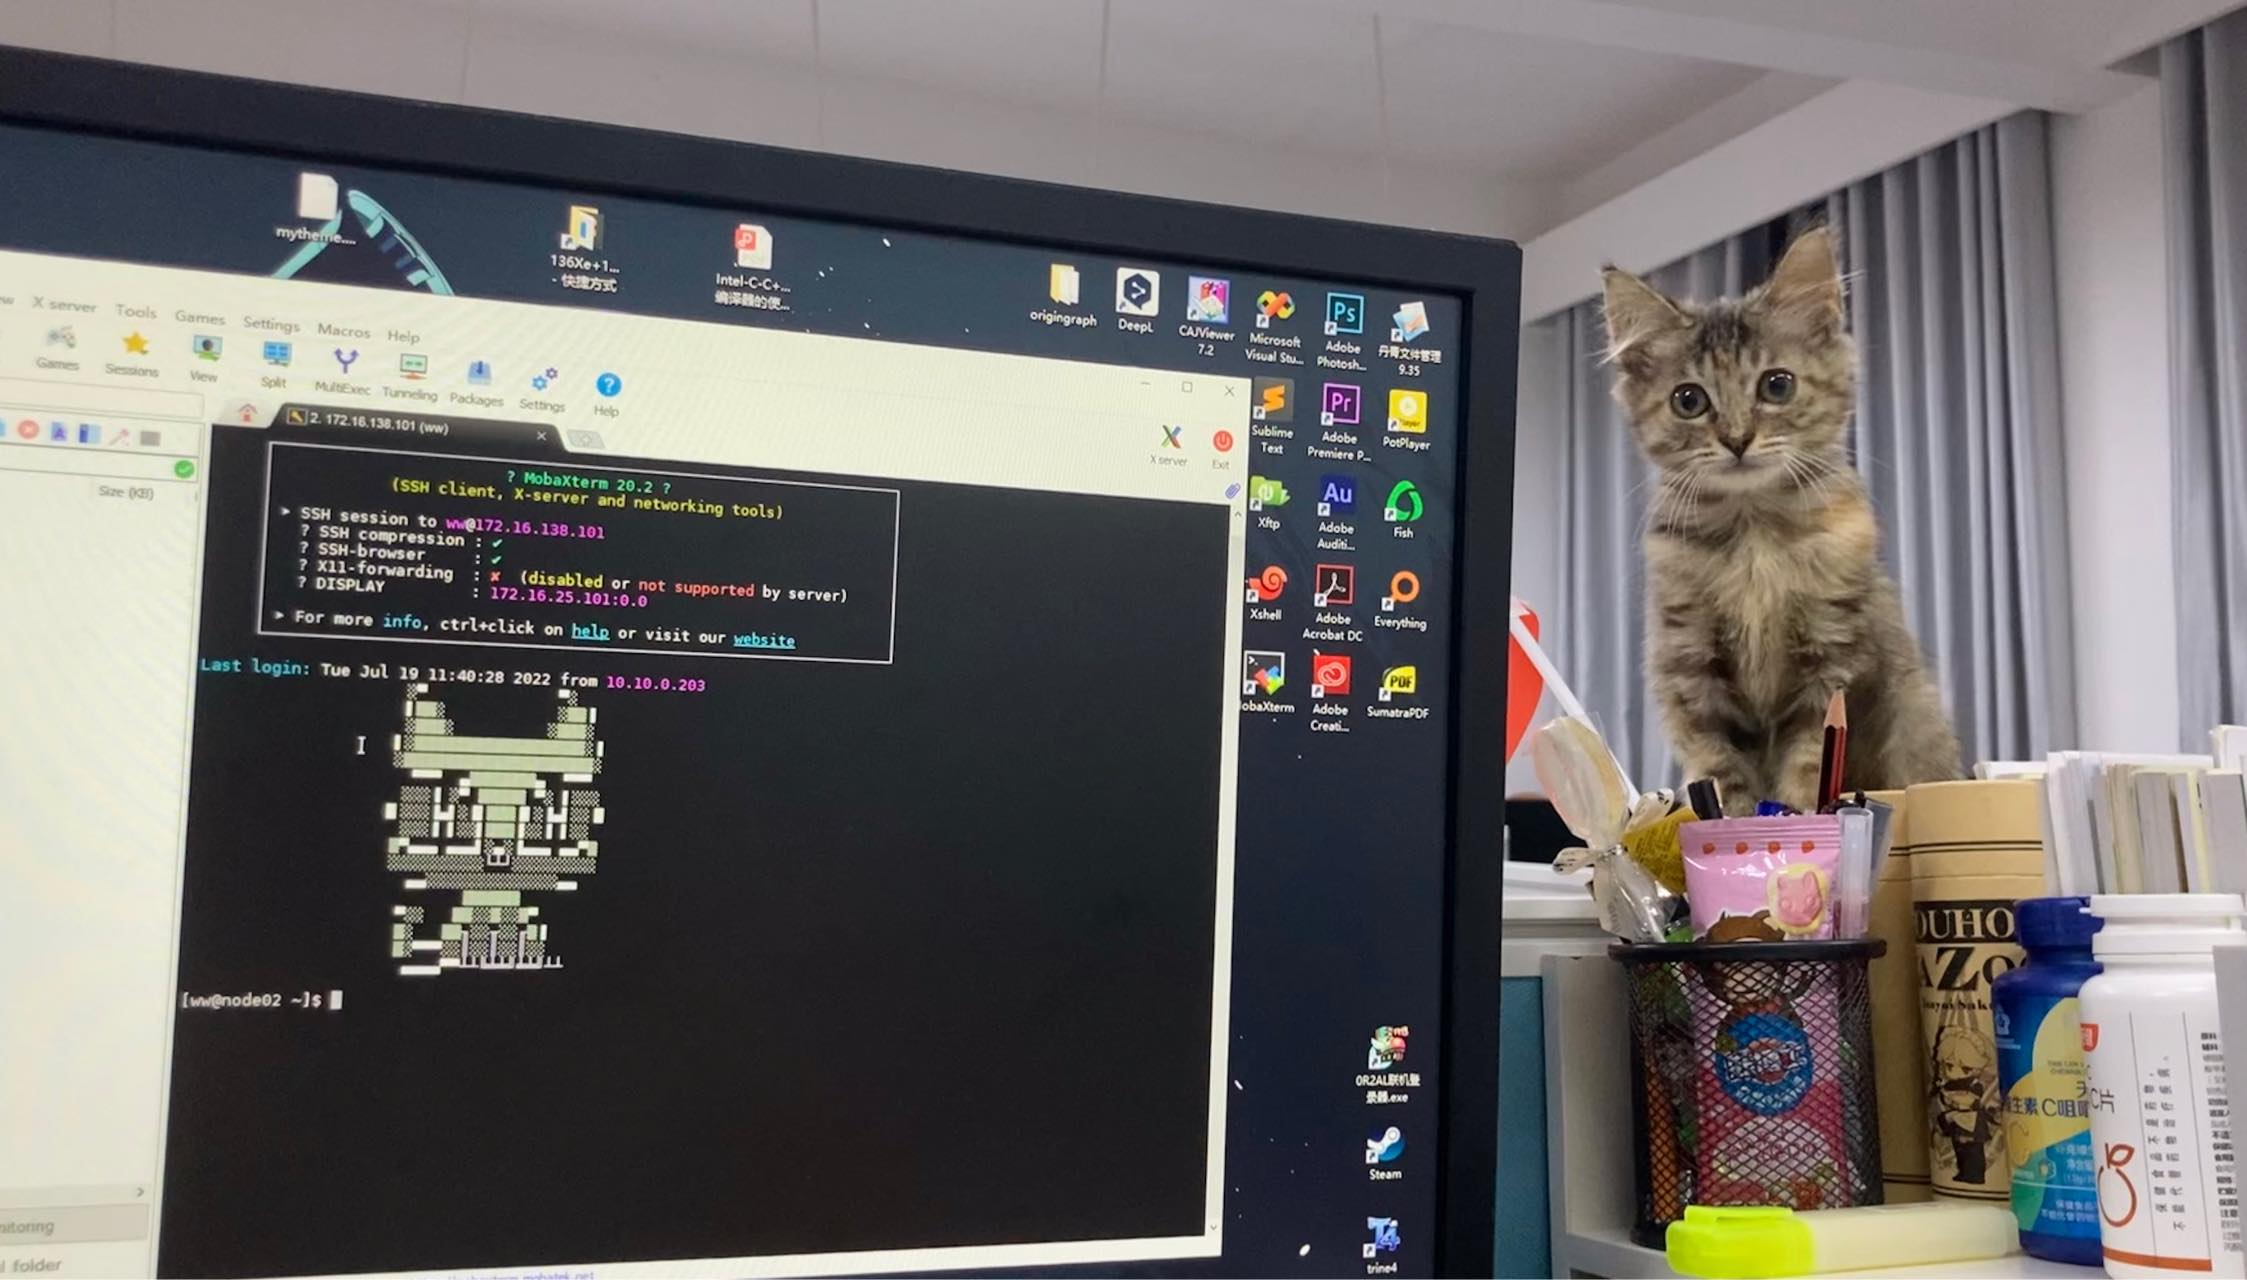
\includegraphics[width=0.76\linewidth]{figures/xuemi.jpg}
	% \caption{}
	\label{xuemi}
\end{figure*}

最后,感谢当年选择物理专业的那个自己。一路走来,世界很美好。
\end{flushleft}



% \pagestyle{empty}
% \cleardoublepage
\phantomsection
\addcontentsline{toc}{chapter}{论文独创性声明}
\clearpage
\phantomsection
\addcontentsline{toc}{chapter}{论文使用授权声明}
% \newpage
\thispagestyle{empty}
{\songti
\begin{center}
{\xiaoerhao\textbf{论文独创性声明}}
\end{center}
}
\begin{flushleft}
\setlength{\parindent}{2em}
\ \par
本人郑重声明:所提交的学位论文是本人在导师的指导下进行的研究工作及取得的成果。除文中已经注明引用的内容外,本论文不含其他个人或其他机构已经发表或撰写过的研究成果。对本文的研究作出重要贡献的个人和集体,均已在文中以明确方式标明。本人承担本声明的法律责任。\par
\end{flushleft}
\begin{flushright}
研究生签名: \underline{\hspace{2.5cm}}
日~~~~期: \underline{\hspace{2.5cm}}
\end{flushright}
\vspace{2cm}
{\songti
\begin{center}
{\xiaoerhao\textbf{论文使用授权声明}}
\end{center}
}
\begin{flushleft}
\setlength{\parindent}{2em}
\ \par
本人完全了解广西师范大学有关保留、使用学位论文的规定。本人授权广西师范大学拥有学位论文的部分使用权,即:学校有权保留本人所送交学位论文的复印件和电子文档,可以采用影印、缩印或其他复制手段保存论文;学校有权向国家有关部门或机构送交学位论文的复印件和电子版。本人电子文档的内容和纸质论文的内容相一致。除在保密期内的保密论文外,允许论文被查阅和借阅,可以公布(包括刊登)论文的全部或部分内容。论文的公布(包括刊登)授权广西师范大学学位办办理。\par
本学位论文属于:\par
$\Box$保密,在~~~~~~~~~年~~~~~~~月~~~~~~~日解密后适用授权。\par
$\Box$延迟公开,申请延迟至~~~~~~~~~年~~~~~~~月~~~~~~~日后公开。\par
$\Box$公开。\par
\end{flushleft}
\begin{flushright}
论文作者签名: \underline{\hspace{2.5cm}}
日~~~~~~~~期: \underline{\hspace{2.5cm}}\par
指导教师签名: \underline{\hspace{2.5cm}}
日~~~~~~~~期: \underline{\hspace{2.5cm}}\par
论文作者联系电话: \underline{\hspace{2.5cm}}
\,电\,子\,邮\,箱: \underline{\hspace{2.5cm}}\par
\end{flushright}
%%--------------------------------独创性申明-----------------------------------------%

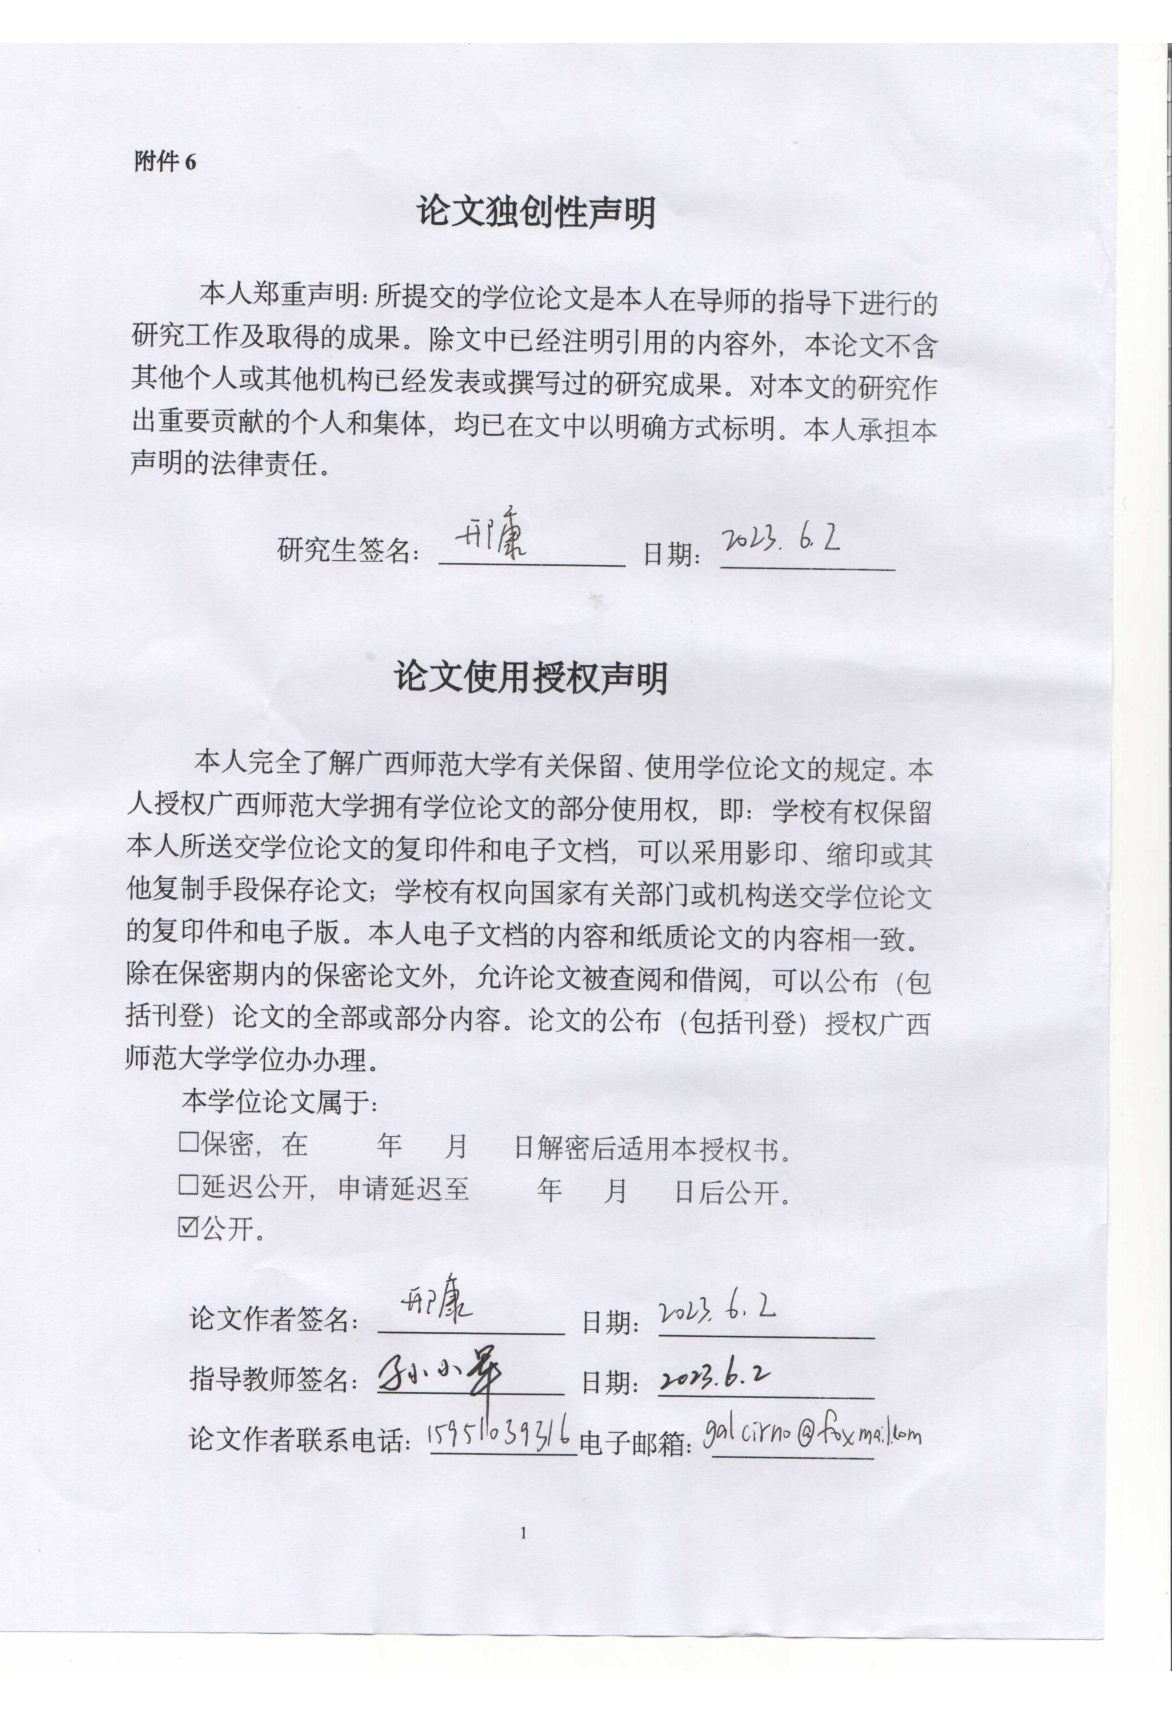
\includepdf{cover/announce.pdf}
\end{spacing}
\end{document}
